\chapter{频率域方法}
\thispagestyle{empty}
\section{频率特性}
\subsection{频率响应}

\tdefination[频率响应]
一个系统的\dy[频率响应]{PLXY}定义为在正弦信号作用下的稳态响应。
\vspace*{1em}

\subsection{频率特性}
令
\begin{align*}
	G(s) = \dfrac{p(s)}{q(s)} = \dfrac{p(s)}{\displaystyle \prod_{i = 1}^n (s - s_i)}\\
	r(t) = A_r \sin \omega t \quad R(s) = \dfrac{A_r\omega}{s^2 + \omega ^2}
\end{align*}
则
\begin{align}
	C(s) = G(s)R(s) = \dfrac{p(s)}{\displaystyle \prod_{i = 1}^n (s - s_i)} \cdot \dfrac{A_r\omega}{s^2 + \omega ^2} = \dfrac{k_1}{s - s_1} + \dfrac{k_2}{s-s_2} + \cdots +\dfrac{k_n}{s - s_n} + \dfrac{a}{s + \j \omega} + \dfrac{\overline{a}}{s - \j \omega}
\end{align}
由Laplace逆变换,
\begin{align}
	c(t) = \sum_{i = 1}^n k_i\e^{s_i t} + a\e^{-\j \omega t} + \overline{a} \e ^{\j \omega t} = c_{\text{t}}(t) + c_{\text{s}}(t)
\end{align}
其中,瞬态分量为
\begin{align}
	c_{\text{t}}(t) = \sum_{i = 1}^n k_i \e^{s_it}
\end{align}
若系统是稳定的,$s_i$均具有负实部,因此$\lim\limits_{t \to 0} c_{\text{t}} (t) = 0$.则稳态分量为
\begin{align}
	c_{\text{s}} = a \e^{- \j \omega t} + \overline{a} \e^{\j \omega t}
\end{align}
记
\begin{align}
	G(\j \omega )= \left|G(\j \omega )\right|\e^{\j \phi}
\end{align}
其中
\begin{align*}
	\phi = \angle G(\j \omega) = \arctan \left[\dfrac{\text{Im}\,G(\j \omega) }{\text{Re} \,G(\j \omega )}\right]
\end{align*}
同理
\begin{align}
	G(-\j \omega) = \left|G(-\j \omega )\right| \e^{-\j \phi}= \left|G(\j \omega )\right|\e^{-\j \phi}
\end{align}

由Laplace逆变换,可得
\begin{align}
	a &= \left. G(s)\dfrac{A_r \omega}{s^2 + \omega^2}(s + \j \omega)\right|_{s = -\j \omega} = -G(- \j \omega )\cdot \dfrac{A_r}{2 \j} = - \dfrac{A_r \big|G(\j \omega)\big|\e^{-\j \phi}}{2\j}\\
	\overline{a} &=  \left. G(s)\dfrac{A_r \omega}{s^2 + \omega^2}(s - \j \omega)\right|_{s = \j \omega} = G( \j \omega )\cdot \dfrac{A_r}{2 \j} =  \dfrac{A_r \big|G(\j \omega)\big|\e^{\j \phi}}{2\j}
\end{align}
代入稳态分量,得
\begin{align}
	c_{\text{s}}(t) &= \dfrac{A_r \big|G(\j \omega)\big|}{2 \j}\left(\e^{\j (\omega + \phi)} - \e^{- \j (\omega + \phi)}\right)\notag\\
	& = A_r \big|G(\j \omega)\big|\dfrac{\e^{\j (\omega + \phi)} - \e^{- \j (\omega + \phi)}}{2 \j}\notag\\
	& = A_r \big|G(\j \omega)\big| \sin(\omega t + \phi)\\
	& = A_\text{c} \sin (\omega t + \phi)
\end{align}
 其中,
 \begin{myitemize}
 	\item $A_\text{c} = A_r \big|G(\j \omega)\big|$\vspace*{-0.5em}
 	\item $\phi = \angle G(\j \omega)$\vspace*{0.3em}
 \end{myitemize}
\vspace*{0.5em}
所以可以看出:对一个稳定的LTI系统,若输入为一个正弦信号,则稳态输出必然是一个同频率的稳定信号,幅值是输入幅值的$\big|G(\j \omega)\big|$倍,输出与输入的相位差为$\angle G(\j \omega)$.
\vspace*{0.5em}

\defination[频率特性]
在正弦信号作用下,LTI系统输出稳态分量的幅值与输入幅值之比,称为这个系统的\dy[幅频特性]{FPTX},用$A(\omega)$表示。稳态输出与输入的相位差,称为系统的\dy[相频特性]{XPTX},用$\varphi(\omega)$表示。即
\vspace*{0.5em}
\begin{align}
	A(\omega) &= \dfrac{A_{\text{c}}}{A_{\text{r}}} = \dfrac{\big|G(\j \omega)\big|A_\text{r}}{A_\text{r}} = \big|G(\j \omega)\big|\\
	\varphi(\omega) &= (\omega t + \phi - \omega t) = \phi = \angle G(\j \omega)
\end{align}

\noindent 幅频特性和相频特性统称为系统的\dy[频率特性]{PLTX},可表示为
\begin{align}
	G(\j \omega) = A(\omega) \e^{\j \omega}
\end{align}
\vspace*{-3em}

\warn[
关于频率特性的几点说明\vspace*{-0.5em}
\begin{enumerate}
	\item 频率特性的对象不只是系统,对控制元件、部件、控制装置也适用\vspace*{-0.5em}
	\item 频率特性只适用于LTI系统\vspace*{-0.5em}
	\item 频率特性研究的是稳态分量,与系统是否稳定无关\vspace*{-0.5em}
	\item 频率特性包含了系统或元部件的全部结果和参数,反映了动态过程的规律性
\end{enumerate}
]

\subsection{频率特性的几何表示方法}
\begin{enumerate}
	\item \textbf{幅频特性曲线}\\
	\hspace*{2em} 以频率$\omega$为横坐标,以幅频$A(\omega)$为纵坐标,画出$A(\omega )$随频率$\omega$变化的曲线,称为\dy[幅频特性曲线]{FPTXQX}。
	
	\item \textbf{相频特性曲线}\\
	\hspace*{2em} 以频率$\omega$为横坐标,以相频$\varphi (\omega)$为纵坐标,画出$\varphi (\omega )$随频率$\omega$变化的曲线,称为\dy[相频特性曲线]{XPTXQX}。
	
	\item \textbf{幅相特性曲线}\\
	\hspace*{2em} 将频率$\omega$作为参变量,将幅频与相频特性同时表示在复数平面上。
	\begin{enumerate}[\hspace*{2em} $-$]
		\item 实轴正方向为相角的零度线,逆时针方向转过的角度为正角度,顺时针方向转过的角度为负角度
		\item 复平面上一个点到原点的距离为幅度
	\end{enumerate}
	由一个确定的频率,必有一个幅值和相角与之对应,由此确定唯一向量。当频率$\omega: 0 \to \infty$时,向量的端点在复数平面上画出一条曲线,称为\dy[幅相特性曲线]{FXTXQX},也称为\dy[奈奎斯特曲线]{NGSTQX}(Nyquist)\index{Nyquist@Nyquist曲线},如图\ref{那奎斯特图}.
	
	\item \textbf{对数频率特性}\\
	\dy[对数频率特性曲线]{DSPLTXQS}又称为\dy[伯德图]{BDT}(Bode)\index{Bode},如图\ref{bode图}.它包括对数幅频与对数相频两条特性曲线。\vspace*{-0.5em}	
	\begin{enumerate}
		\item 对数幅频特性曲线
		\begin{itemize}
			\item 纵坐标\quad 幅频$A(\omega)$取以10为底的对数后再乘以20的值,即$L(\omega) = 20 \lg \big( A(\omega) \big)$,\\ 单位为db(分贝),采用线性刻度。
			\item 横坐标 \quad 角频率$\omega$,按对数$\lg \omega $刻度,但标注为真实$\omega$值。因此,频率每变化十倍,横坐标轴上就变化一个单位长度,称为“十倍频程”。对数刻度是不均匀刻度。
		\end{itemize}
		
		\item 对数相频特性
		\begin{itemize}
			\item 纵坐标 \quad 相频$\varphi(\omega)$的值,线性刻度,单位为$\degree$(度)或rad(弧度)。
			\item 横坐标 \quad 与对数幅频特性曲线的横坐标相同。
		\end{itemize}
	\end{enumerate}
\end{enumerate}
\begin{figure}[!htb]
		\begin{minipage}{0.45\linewidth}
		\centering
		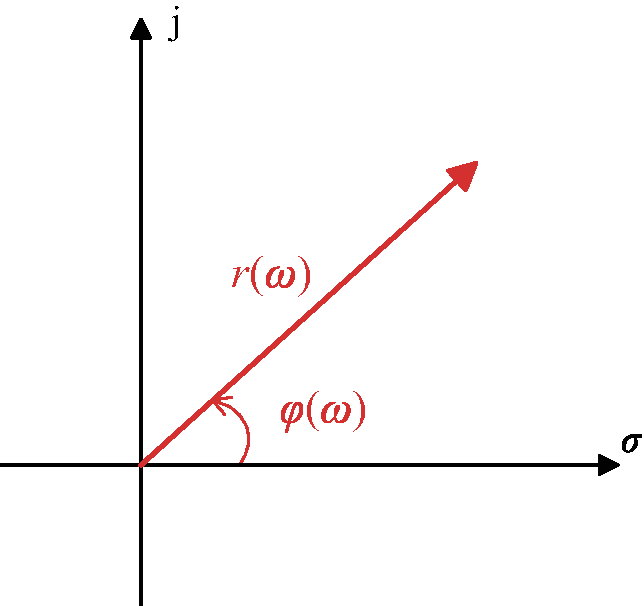
\includegraphics[width=0.9\linewidth]{pic/那奎斯特图.pdf}
		\caption{那奎斯特图}
		\label{那奎斯特图}
	\end{minipage}
	\begin{minipage}{0.55\linewidth}
		\centering
		\includegraphics[width=0.9\linewidth]{pic/bode图.png}
		\vspace*{-0.2em}
		\caption{伯德图}
		\label{bode图}
	\end{minipage}
\end{figure}

\newpage
\noindent 利用Bode 图及Nyquist图,我们可以
\begin{itemize}
	\item 方便地确定系统在不同频率下的响应
	\item 分析系统的闭环稳定性
	\item 基于频率特性设计控制器,改善系统性能
	\item 将频率特性方法拓展到某些非线性系统。
\end{itemize}


\section{典型环节的频率特性}
\subsection{比例环节}
\begin{enumerate}[1.]
	\item 传递函数
	\vspace*{-0.5em}
	\begin{align}
		G(s) = K
	\end{align}
	\vspace*{-3em}
	
	\item 频率特性
	\vspace*{-0.5em}
	\begin{align}
		G(j\omega) = K
	\end{align}
	\vspace*{-3em}
	\begin{enumerate}[(1) ]
		\item 幅频特性
		\vspace*{-0.5em}
		\begin{align}
			A(\omega) = K
		\end{align}
		\vspace*{-3em}
		
		\item 相频特性
		\vspace*{-0.5em}
		\begin{align}
			\varphi(\omega) = 0
		\end{align}
		\vspace*{-3em}
	\end{enumerate}
		\item 对数频率特性
	\begin{enumerate}[(1) ]
		\item 对数幅频特性
		\vspace*{-0.5em}
		\begin{align}
			L(\omega) = 20 \lg K
		\end{align}
		\vspace*{-3em}
		\item 对数相频特性
		\vspace*{-0.5em}
		\begin{align}
			\varphi(\omega) = 0
		\end{align}
		\vspace*{-3em}
	\end{enumerate}
\end{enumerate}


\subsection{积分环节}
\begin{enumerate}[1.]
	\item 传递函数
	\vspace*{-0.5em}
	\begin{align}
		G(s) = \dfrac{1}{s}
	\end{align}
	\vspace*{-3em}
	
	\item 幅相特性
	\vspace*{-0.5em}
	\begin{align}
		G(\j  \omega) = \dfrac{1}{\j \omega}
	\end{align}
	\vspace*{-3em}
	\begin{enumerate}[(1) ]
		\item 频率特性
		\vspace*{-0.5em}
		\begin{align}
			A(\omega) = \dfrac{1}{\omega}
		\end{align}
		\vspace*{-3em}
		
		\item 相频特性
		\vspace*{-0.5em}
		\begin{align}
			\textcolor{red}{\varphi(\omega) =  \arctan \left(\dfrac{\omega}{0}\right)}
		\end{align}
		\vspace*{-3em}
		
		\item 幅相特性
		\vspace*{-0.5em}
		\begin{align}
			G(\j \omega) = \dfrac{1}{\omega} \e^{- \j  \arctan \left(\frac{\omega}{0}\right)}
		\end{align}
		\vspace*{-3em}
	\end{enumerate}
	\item 对数频率特性
	\begin{enumerate}[(1) ]
		\item 对数幅频特性
		\vspace*{-0.5em}
		\begin{align}
			L(\omega) = 20 \lg A(\omega) = 20 \lg \dfrac{1}{\omega} = - 20 \lg \omega
		\end{align}
		\vspace*{-0.5em}
		\textbf{积分环节的对数幅频是斜率为$-$20db/dec(分贝/十倍频程)的直线。}
		\item 对数相频特性
		\vspace*{-0.5em}
		\begin{align}
			\textcolor{red}{\varphi(\omega) = \arctan \left(\dfrac{\omega}{0}\right) = \text{sign}(\omega) \cdot 90 \degree = \, 
			\begin{cases}
				\, 90 \degree, & \omega >0 \quad \mbox{(特别是}0^+\mbox{)}\\
				\, 0 \degree, & \omega = 0\\
				\, -90 \degree, & \omega <0 \quad \mbox{(特别是}0^-,-\infty\mbox{)}
		\end{cases}}
		\end{align}
		\vspace*{-3em}
	\end{enumerate}
\end{enumerate}


\subsection{一阶环节}
\begin{enumerate}[1.]
	\item 传递函数
	\vspace*{-0.5em}
	\begin{align}
		G(s) = \dfrac{1}{Ts + 1}
	\end{align}
	\vspace*{-3em}
	
	\item 频率特性
	\vspace*{-0.5em}
	\begin{align}
		G(\j  \omega) = \dfrac{1}{T \j \omega + 1}
	\end{align}
	\vspace*{-3em}
	\begin{enumerate}[(1) ]
		\item 幅频特性
		\vspace*{-0.5em}
		\begin{align}
			A(\omega) = \dfrac{1}{\sqrt{(T\omega)^2 + 1}}
		\end{align}
		\vspace*{-3em}
		
		\item 相频特性
		\begin{align}
			\varphi(\omega) = -\arctan T\omega
		\end{align}
		\vspace*{-3em}
		
		\item 幅相特性
		\vspace*{-0.5em}
		\begin{align}
			G(\j \omega) = \dfrac{1}{\sqrt{(T\omega)^2 + 1}} \e^{-j  \arctan T\omega}
		\end{align}
		\vspace*{-3em}
		
	\end{enumerate}
	\item 对数频率特性
	\begin{enumerate}[(1) ]
		\item 对数幅频特性
		\vspace*{-0.5em}
		\begin{align}
			L(\omega) = 20 \lg A(\omega) = 20 \lg \left[\dfrac{1}{\sqrt{(T \omega)^2 + 1}}\right] = -20 \lg \left[\sqrt{(T \omega)^2 + 1}\right]
		\end{align}
		其渐近线表达式为
		\begin{align}
			L(\omega) = \,
			\begin{cases}
				\, -20 \lg 1 = 0 \text{dB}, & \omega < \dfrac{1}{T}\\[0.5em]
				\, -20 \lg T\omega = - 20 \lg \dfrac{\omega}{\omega_\n} , & \omega > \dfrac{1}{T}
			\end{cases}
		\end{align}
		转折频率$\omega = \dfrac{1}{T}$, 斜率$-$20dB/dec,最大误差为转折频率处,大约为3dB.
		\item 对数相频特性
		\vspace*{-0.5em}
		\begin{align}
			\varphi(\omega) = -\arctan T\omega = \,
			\begin{cases}
				\, 0, & \omega = 0\\[0.5em]
				\, -45\degree , & \omega = \dfrac{1}{T}\\[0.5em]
				\, -90 \degree, & \omega \to \infty
			\end{cases}
		\end{align}
		\vspace*{-3em}
		
		特点
		\begin{itemize}
			\item 在转折频率$\omega = \dfrac{1}{T}$处,$\varphi(\omega) =  -\dfrac{\pi}{4}$,且曲线对$-\dfrac{\pi}{4}$具有奇对称性。
			\item 当改变时间常数$T$时,转折频率向左或右移动,曲线形状不变。
		\end{itemize}
	\end{enumerate}
\end{enumerate}


\subsection{二阶环节}
\begin{enumerate}[1.]
	\item 传递函数
	\vspace*{-0.5em}
	\begin{align}
		G(s) = \dfrac{\omega_n^2}{s^2 + 2 \zeta \omega_ns + \omega_n^2}
	\end{align}
	\vspace*{-3em}
	
	\item 频率特性
	\vspace*{-0.5em}
	\begin{align}
		G(\j  \omega) = \dfrac{\omega_\n^2}{(\j \omega)^2 + 2 \zeta \omega_\n \j \omega + \omega_\n^2}
	\end{align}
	\vspace*{-3em}
	\begin{enumerate}[(1) ]
		\item 幅频特性
		\vspace*{-0.5em}
		\begin{equation}
			\begin{split}
				A(\omega) &= \dfrac{\omega_\n^2}{\sqrt{\left(\omega_\n^2 - \omega^2\right)^2 + \left(2 \zeta \omega_\n \omega\right)^2}}\\
				& =  \dfrac{1}{\sqrt{\left[1 - \left(\dfrac{\omega}{\omega_\n}\right)^2\right]^2 + \left(2 \zeta \dfrac{\omega}{\omega_\n}\right)^2}}
			\end{split}
		\end{equation}

		幅频曲线的特点
		\begin{itemize}
			\item 两个极限点及转折点
			\begin{align*}
				\lim\limits_{\omega \to 0} A(\omega) = 1\\
				\lim\limits_{\omega \to \infty} A(\omega) = 0\\
				A(\omega_\n) = \dfrac{1}{2 \zeta}
			\end{align*}
		
			\item \dy[谐振频率]{XZPL}
			\begin{align}
				\dfrac{\d A(\omega)}{\d \omega} = 0 \quad \Rightarrow \quad \omega_\text{m} = \omega_\n \sqrt{1 - 2 \zeta^2}, \quad 0< \zeta < \dfrac{\sqrt{2}}{2}
				\label{谐振频率}
			\end{align}
		
			\item \dy[谐振峰值]{XZFZ}
			\begin{align}
				A_\text{m} = A(\omega_\text{m}) = \dfrac{1}{2 \zeta \sqrt{1-\zeta^2}}
				\label{谐振峰值}
			\end{align}
			
			
		\end{itemize}
		\item 相频特性
		\begin{align}
			\varphi(\omega) = -\arctan \left[\dfrac{2 \zeta \dfrac{\omega}{\omega_\n}}{1 - \left(\dfrac{\omega}{\omega_\n}\right)^2}\right]
		\end{align}
		\vspace*{-1em}
		
		\item 幅相特性
		\vspace*{-0.5em}
		\begin{align}
			G(\j \omega) = \dfrac{1}{\sqrt{\left[1 - \left(\dfrac{\omega}{\omega_\n}\right)^2\right]^2 + \left(2 \zeta \dfrac{\omega}{\omega_\n}\right)^2}} \exp\left\lbrace-\j \arctan \left[\dfrac{2 \zeta \dfrac{\omega}{\omega_\n}}{1 - \left(\dfrac{\omega}{\omega_\n}\right)^2}\right]\right\rbrace
		\end{align}
		\vspace*{-3em}
		
	\end{enumerate}
	\item 对数频率特性
	\begin{enumerate}[(1) ]
		\item 对数幅频特性
		\vspace*{-0.5em}
		\begin{equation}
			\begin{split}
				L(\omega) & = 20\lg A(\omega) = 20 \lg \dfrac{1}{\sqrt{\left[1 - \left(\dfrac{\omega}{\omega_\n}\right)^2\right]^2 + \left(2 \zeta \dfrac{\omega}{\omega_\n}\right)^2}}\\[0.5em]
				& = -20 \lg \sqrt{\left[1 - \left(\dfrac{\omega}{\omega_\n}\right)^2\right]^2 + \left(2 \zeta \dfrac{\omega}{\omega_\n}\right)^2}
			\end{split}
		\end{equation}
		其渐近线表达式为
		\begin{align}
			L(\omega) = \,
			\begin{cases}
				\, -20 \lg 1 = 0 \text{dB}, & \omega < \omega_\n\\[0.5em]
				\, -20 \lg \left(\dfrac{\omega}{\omega_\n}\right)^2= - 40 \lg \dfrac{\omega}{\omega_\n}, & \omega > \omega_\n
			\end{cases}
		\end{align}
		转折频率$\omega = \omega_\n$, 斜率$-$40dB/dec,转折频率处的误差为$\dfrac{1}{2 \zeta }$。\textcolor{red}{最大误差为谐振频率处,为$ \dfrac{1}{2 \zeta \sqrt{1-\zeta^2}}$.}
		\item 对数相频特性
		\vspace*{-0.5em}
		\begin{align}
			\varphi(\omega) = \varphi(\omega) = -\arctan \left[\dfrac{2 \zeta \dfrac{\omega}{\omega_\n}}{1 - \left(\dfrac{\omega}{\omega_\n}\right)^2}\right] = \,
			\begin{cases}
				\, 0, & \omega = 0\\[0.5em]
				\, -90\degree , & \omega = \omega_\n\\[0.5em]
				\, -180 \degree, & \omega \to \infty
			\end{cases}
		\end{align}
		\vspace*{-3em}
		
		特点
		\begin{itemize}
			\item 在转折频率$\omega = \omega_\n$处,$\varphi(\omega) =  -\dfrac{\pi}{2}$,且曲线对$-\dfrac{\pi}{2}$具有奇对称性。
			\item 当改变常数$\omega_\n$时,转折频率向左或右移动,曲线形状不变。
		\end{itemize}
	\end{enumerate}
\end{enumerate}

\subsection{微分环节}
\begin{enumerate}[1.]
	\item 传递函数
	\vspace*{-0.5em}
	\begin{align}
		G(s) = s
	\end{align}
	\vspace*{-3em}
	
	\item 频率特性
	\vspace*{-0.5em}
	\begin{align}
		G(j\omega) = \j \omega 
	\end{align}
	\vspace*{-3em}
	\begin{enumerate}[(1) ]
		\item 幅频特性
		\vspace*{-0.5em}
		\begin{align}
			A(\omega) = \omega
		\end{align}
		\vspace*{-3em}
		
		\item 相频特性
		\vspace*{-0.5em}
		\begin{align}
			\varphi(\omega) = \dfrac{\pi}{2}
		\end{align}
		\vspace*{-3em}
	\end{enumerate}
	\item 对数频率特性
	\begin{enumerate}[(1) ]
		\item 对数幅频特性
		\vspace*{-0.5em}
		\begin{align}
			L(\omega) = 20 \lg \omega
		\end{align}
		\vspace*{-3em}
		\item 对数相频特性
		\vspace*{-0.5em}
		\begin{align}
			\varphi(\omega) = \dfrac{\pi}{2}
		\end{align}
		\vspace*{-3em}
	\end{enumerate}
\end{enumerate}

\subsection{一阶微分环节}

\begin{enumerate}[1.]
	\item 传递函数
	\vspace*{-0.5em}
	\begin{align}
		G(s) = \tau s + 1
	\end{align}
	\vspace*{-3em}
	
	\item 频率特性
	\vspace*{-0.5em}
	\begin{align}
		G(\j  \omega) = \tau \j \omega + 1
	\end{align}
	\vspace*{-3em}
	\begin{enumerate}[(1) ]
		\item 幅频特性
		\vspace*{-0.5em}
		\begin{align}
			A(\omega) = \sqrt{(\tau \omega)^2 + 1}
		\end{align}
		\vspace*{-3em}
		
		\item 相频特性
		\begin{align}
			\varphi(\omega) = \arctan \tau \omega
		\end{align}
		\vspace*{-3em}
		
		\item 幅相特性
		\vspace*{-0.5em}
		\begin{align}
			G(\j \omega) = \sqrt{(\tau \omega)^2 + 1}\e^{-j  \arctan T\omega}
		\end{align}
		\vspace*{-3em}
		
	\end{enumerate}
	\item 对数频率特性\\
	\textbf{一阶微分环节的对数幅频和对数相频特性表达式与一阶环节相比仅相差一个符号,所以它们的曲线关于频率轴对称。}
	\begin{enumerate}[(1) ]
		\item 对数幅频特性
		\vspace*{-0.5em}
		\begin{align}
			L(\omega) = 20 \lg A(\omega) = 20 \lg \sqrt{(\tau \omega)^2 + 1}
		\end{align}
		
		转折频率$\omega = \dfrac{1}{T}$, 斜率20dB/dec,最大误差为转折频率处,大约为3dB.
		\item 对数相频特性
		\vspace*{-0.5em}
		\begin{align}
			\varphi(\omega) =  \arctan \tau \omega = \,
			\begin{cases}
				\, 0, & \omega = 0\\[0.5em]
				\, 45\degree , & \omega = \dfrac{1}{\tau}\\[0.5em]
				\, 90 \degree, & \omega \to \infty
			\end{cases}
		\end{align}
		\vspace*{-3em}
	\end{enumerate}
\end{enumerate}

\subsection{二阶微分环节}
\begin{enumerate}[1.]
	\item 传递函数
	\vspace*{-0.5em}
	\begin{align}
		G(s) = \left(\dfrac{s}{\omega_\n}\right)^2 + 2 \zeta \dfrac{s}{\omega_\n} + 1
	\end{align}
	\vspace*{-3em}
	
	\item 频率特性
	\vspace*{-0.5em}
	\begin{align}
		G(\j  \omega) =  \left(\dfrac{\j \omega}{\omega_\n}\right)^2 + 2 \zeta \dfrac{\j \omega }{\omega_\n} + 1
	\end{align}
	\vspace*{-3em}
	\begin{enumerate}[(1) ]
		\item 幅频特性
		\vspace*{-0.5em}
		\begin{equation}
			A (\omega) = \sqrt{\left[1 - \left(\dfrac{\omega}{\omega_\n}\right)^2\right]^2 + \left(2 \zeta \dfrac{\omega}{\omega_\n}\right)^2}
		\end{equation}
			
		\item 相频特性
		\begin{align}
			\varphi(\omega) = \arctan \left[\dfrac{2 \zeta \dfrac{\omega}{\omega_\n}}{1 - \left(\dfrac{\omega}{\omega_\n}\right)^2}\right]
		\end{align}
		\vspace*{-1em}
		
		\item 幅相特性
		\vspace*{-0.5em}
		\begin{align}
			G(\j \omega) = \sqrt{\left[1 - \left(\dfrac{\omega}{\omega_\n}\right)^2\right]^2 + \left(2 \zeta \dfrac{\omega}{\omega_\n}\right)^2} \exp\left\lbrace \j \arctan \left[\dfrac{2 \zeta \dfrac{\omega}{\omega_\n}}{1 - \left(\dfrac{\omega}{\omega_\n}\right)^2}\right]\right\rbrace
		\end{align}
		\vspace*{-3em}
		
	\end{enumerate}
	\item 对数频率特性\\
	\textbf{二阶微分环节的对数幅频和对数相频特性表达式与二阶环节相比仅相差一个符号,所以它们的曲线关于频率轴对称。}
	\begin{enumerate}[(1) ]
		\item 对数幅频特性
		\vspace*{-0.5em}
		\begin{equation}
			L(\omega)  = 20\lg A(\omega) = 20 \lg \sqrt{\left[1 - \left(\dfrac{\omega}{\omega_\n}\right)^2\right]^2 + \left(2 \zeta \dfrac{\omega}{\omega_\n}\right)^2}\\[0.5em]
		\end{equation}
		转折频率$\omega = \omega_\n$, 斜率40dB/dec,最大误差为转折频率处,为$2\zeta$.
		\item 对数相频特性
		\vspace*{-0.5em}
		\begin{align}
			\varphi(\omega) = \varphi(\omega) = \arctan \left[\dfrac{2 \zeta \dfrac{\omega}{\omega_\n}}{1 - \left(\dfrac{\omega}{\omega_\n}\right)^2}\right] = \,
			\begin{cases}
				\, 0, & \omega = 0\\[0.5em]
				\, 90\degree , & \omega = \omega_\n\\[0.5em]
				\, 180 \degree, & \omega \to \infty
			\end{cases}
		\end{align}
		\vspace*{-3em}
	\end{enumerate}
\end{enumerate}

\subsection{一阶不稳定环节}
\begin{enumerate}[1.]
	\item 传递函数
	\vspace*{-0.5em}
	\begin{align}
		G(s) =  \dfrac{1}{Ts - 1}
	\end{align}
	\vspace*{-2em}
	
	其中,$T>0,s_1 = \dfrac{1}{T} > 0$,所以环节是不稳定的。
	
	\item 频率特性
	\vspace*{-0.5em}
	\begin{align}
		G(j\omega) = \dfrac{1}{T \j \omega - 1}
	\end{align}
	\vspace*{-3em}
	\begin{enumerate}[(1) ]
		\item 幅频特性
		\vspace*{-0.5em}
		\begin{align}
			A(\omega) = \dfrac{1}{\sqrt{(\j \omega)^2 + 1}}
		\end{align}
		\vspace*{-3em}
		
		\item 相频特性
		\vspace*{-0.5em}
		\begin{align}
			\varphi(\omega) = - \arctan(- T \omega)
		\end{align}
		\vspace*{-3em}
	\end{enumerate}
	\item 对数频率特性\\
	\textbf{一阶不稳定环节的对数幅频特性与一阶环节完全一致,而相频特性不一致。}
	\begin{enumerate}[(1) ]
		\item 对数幅频特性
		\vspace*{-0.5em}
		\begin{align}
			L(\omega) = - 20 \lg \sqrt{(T\omega)^2 + 1}
		\end{align}
		\vspace*{-2em}
		
		转折频率$\omega = \dfrac{1}{T}$, 斜率$-$20dB/dec,最大误差为转折频率处。
		
		\item 对数相频特性
		\vspace*{-0.5em}
		\begin{align}
			\varphi(\omega) = - \arctan(- T \omega) = \,
			\begin{cases}
				\, -180, & \omega = 0\\[0.5em]
				\, -135\degree , & \omega = \dfrac{1}{T}\\[0.5em]
				\, -90 \degree, & \omega \to \infty
			\end{cases}
		\end{align}
		\vspace*{-1em}
		
		当$\omega: 0 \to \infty$时,一阶环节的相频$\varphi(\omega ): 0 \to -90\degree$,而一阶不稳定环节的相频$\varphi(\omega ): -180 \to -90\degree$,所以一阶环节常称为\dy[最小相位环节]{ZXXWHJ},一阶不稳定系统常称为\dy[非最小相位环节]{FZXXWHJ}。
	\end{enumerate}
\end{enumerate}

\vspace*{-1em}
\warn[
{
\begin{enumerate}[1. ]
	\item 对最小相位系统,传递函数可由幅频特性曲线唯一确定;但非最小相位系统的传递函数则不能仅由幅频特性曲线决定。\vspace*{-0.5em}
	
	\item 对具有相同幅频特性的系统,最小相位系统的相角变化范围是最小的。\vspace*{-0.5em}
	
	\item 在计算角度时,设所有的环节都满足$0\degree \le \theta \le 180 \degree$,则 $\arctan(-T\omega) = 180 \degree - \arctan(T \omega)$,对于非最小相位环节需要做这个处理。
\end{enumerate}
}
]

\section{系统的开环频率特性}

\subsection{开环幅相特性曲线}

考虑一般形式$(n < m)$
\begin{align}
	G(\j \omega) = \dfrac{\displaystyle \prod_{i=1}^{m} \left(1 + \j \omega \tau_i \right)}{\displaystyle \left(\j \omega\right)^{\lambda} \prod_{i=1}^{n - \lambda} \left(1 + \j \omega T_i \right) }, \quad \lambda = 0,1,2
\end{align}

绘制概略幅相特性曲线时,一般要分别考虑低频段$(\omega = 0)$和高频段$(\omega \to \infty)$时的幅值和相角特点。

\begin{enumerate}[1.]
	\item \textbf{$\bm{\lambda}\,  \mathbf{= 0}$, Type 0 系统}
	
	\examples \label{5.1}考虑如下开环传递函数:
	\begin{align*}
		G(s) = \dfrac{K}{(T_1 s + 1)(T_2 s + 1)}
	\end{align*}
	绘概略幅相特性曲线,其中$T_1,T_2 > 0$.
	
	\solve 频率特性函数为
	\begin{align*}
		G(\j \omega) = \dfrac{K}{(T_1 \j \omega + 1)(T_2 \j \omega + 1)}
	\end{align*}
	其幅频特性与相频特性分别为
	\begin{align*}
		A(\omega) &= \dfrac{K}{\sqrt{(T_1 \omega )^2 + 1} \sqrt{(T_2 \omega)^2 + 1}}\\
		\varphi(\omega) &= - \arctan(T_1 \omega) - \arctan(T_2 \omega)
	\end{align*}
\begin{itemize}
	\item 低频段\quad $\omega = 0 \quad \Rightarrow \quad A(\omega) = K,\quad \varphi(\omega) = 0\degree $
	
	\item 高频段\quad $\omega \to \infty \quad \Rightarrow \quad A(\omega) \to 0,\quad \varphi(\omega) = -90\degree - 90 \degree = -180 \degree$
\end{itemize}
所以其概略幅频特性曲线如图\ref{F5.1}.
\begin{figure}[!htb]
	\centering
	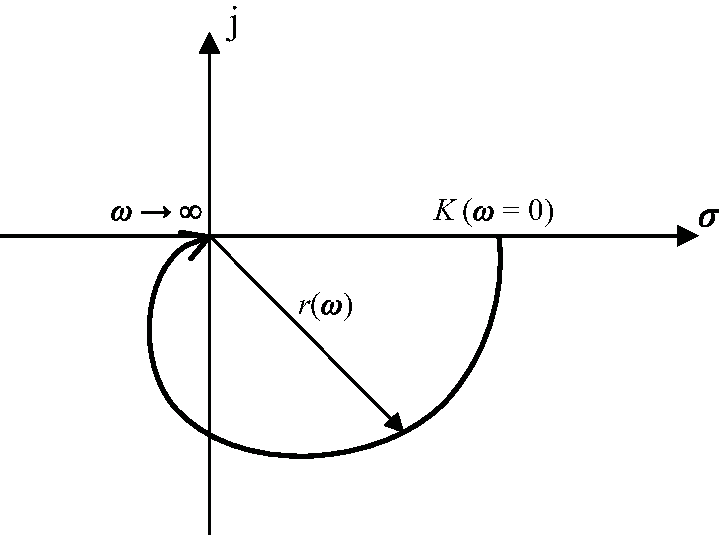
\includegraphics[width=0.45\linewidth]{pic/5.1.pdf}
	\caption{\ref{5.1}$\,$幅频特性曲线}
	\label{F5.1}
\end{figure}

\item \textbf{$\bm{\lambda}\,  \mathbf{= 1}$, Type 1 系统}

\examples \label{5.2}考虑如下开环传递函数:
\begin{align*}
	G(s) = \dfrac{K}{s(T s + 1)}
\end{align*}
绘概略幅相特性曲线,其中$K,T > 0$.

\solve 频率特性函数为
\begin{align*}
	G(\j \omega) = \dfrac{K}{\j \omega (T \j \omega +1)}
\end{align*}
其幅频特性与相频特性分别为
\begin{align*}
	A(\omega) &= \dfrac{K}{\omega \sqrt{(T \omega)^2 + 1}}\\[0.5em]
	\varphi(\omega) &= - \dfrac{\pi}{2} - \arctan(T \omega)
\end{align*}
\begin{itemize}
	\item 低频段\quad $\omega = 0 \quad \Rightarrow \quad A(\omega) = \infty ,\quad \varphi(\omega) = -90\degree $
	
	\item 高频段\quad $\omega \to \infty \quad \Rightarrow \quad A(\omega) \to 0,\quad \varphi(\omega) = -90\degree - 90 \degree = -180 \degree$
\end{itemize}
所以其概略幅频特性曲线如图\ref{F5.2}.
\begin{figure}[!htb]
	\centering
	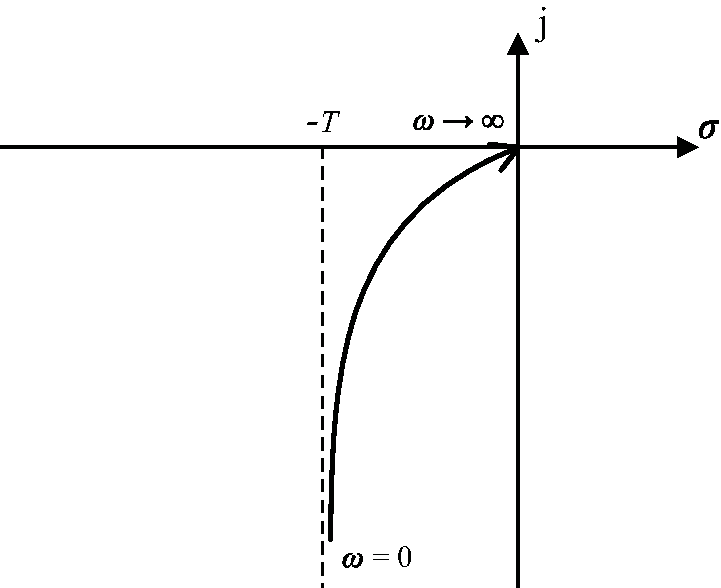
\includegraphics[width=0.4\linewidth]{pic/5.2.pdf}
	\caption{\ref{5.2}$\,$幅频特性曲线}
	\label{F5.2}
\end{figure}

\item \textbf{$\bm{\lambda}\,  \mathbf{= 2}$, Type 2 系统}

\examples \label{5.3}考虑如下开环传递函数:
\begin{align*}
	G(s) = \dfrac{K}{s^2(T s + 1)}
\end{align*}
绘概略幅相特性曲线,其中$K,T > 0$.

\solve 频率特性函数为
\begin{align*}
	G(\j \omega) = \dfrac{K}{(\j \omega)^2 (T \j \omega +1)}
\end{align*}
其幅频特性与相频特性分别为
\begin{align*}
	A(\omega) &= \dfrac{K}{\omega^2 \sqrt{(T \omega)^2 + 1}}\\
	\varphi(\omega) &= - \pi - \arctan(T \omega)
\end{align*}
\begin{itemize}
	\item 低频段\quad $\omega = 0 \quad \Rightarrow \quad A(\omega) = \infty ,\quad \varphi(\omega) = -180\degree $
	
	\item 高频段\quad $\omega \to \infty \quad \Rightarrow \quad A(\omega) \to 0,\quad \varphi(\omega) = -180\degree - 90 \degree = -270 \degree$
\end{itemize}
所以其概略幅频特性曲线如图\ref{F5.3}.
\begin{figure}[!htb]
	\centering
	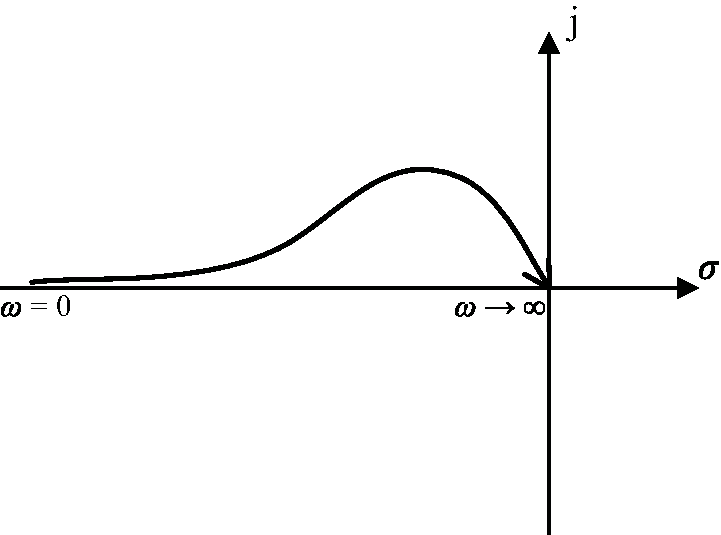
\includegraphics[width=0.45\linewidth]{pic/5.3.pdf}
	\caption{\ref{5.3}$\,$幅频特性曲线}
	\label{F5.3}
\end{figure}

\item 三种系统的总结如图\ref{F5.sum}.\vspace*{-1em}
\begin{figure}[!htb]
	\centering
	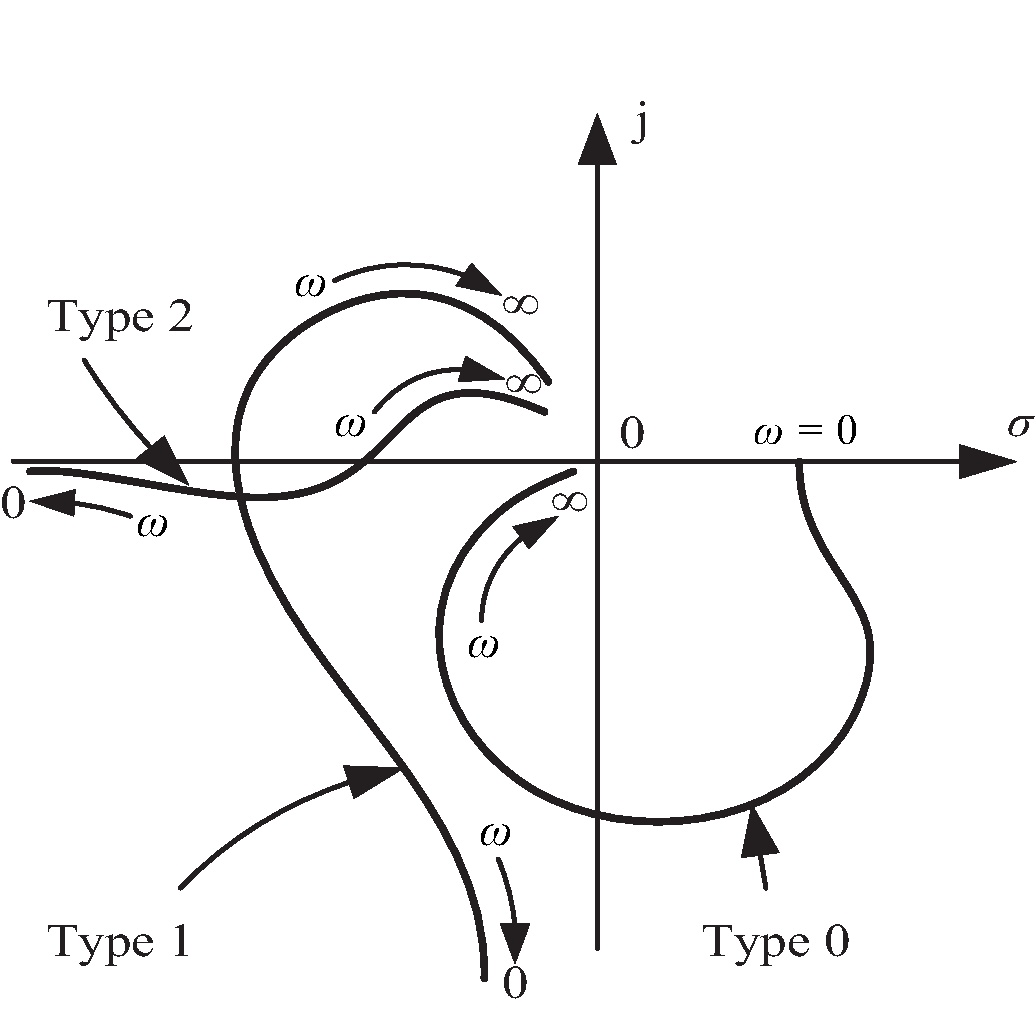
\includegraphics[width=0.45\linewidth]{pic/5.sum.pdf}
	\caption{三种系统的幅频特性曲线总结}
	\label{F5.sum}
\end{figure}
\end{enumerate}

\subsection{开环对数频率特性曲线}

\noindent \textbf{一般规则}:
\begin{itemize}
	\item 将开环传递函数写成各个典型环节之积
	\begin{align}
		G(s) = \dfrac{K (\tau_1 s + 1)(\tau_2 s + 1)}{s(T_1 s + 1)(T_2 s + 1)\left[\left(s/\omega_\n\right)^2 + 2 \zeta \left(s/\omega_\n\right) + 1\right]}
	\end{align}
	
	\item 找出各个环节的转折频率
		$\dfrac{1}{\tau_1}, \quad \dfrac{1}{\tau_2}, \quad \dfrac{1}{T_1}, \quad \dfrac{1}{T_2}, \quad \omega_\n, \quad \cdots $
	
	\item 画出各环节的渐近线及对应的相频特性曲线
	\item 在转角频率处修正渐近线得各环节曲线
	\item 将各环节曲线相加即得Bode图
\end{itemize}

\examples \label{5.4}绘制如下开环传递函数的Bode图:
\begin{align*}
	G(s) = \dfrac{5(0.1s + 1)}{s (0.5s + 1) \left[\left(s/50\right)^2 + 0.6 \left(s/50\right) + 1\right]}
\end{align*}

\solve 传递函数存在以下环节
\begin{itemize}
	\item 比例环节 \quad $K = 5, \quad 20\lg K \approx 14 dB$
	\item 积分环节 \quad $\dfrac{1}{s}$,斜率$-$20dB/dec
	\item 一阶环节 \quad $\dfrac{1}{0.5s + 1}$,转折频率$\omega_{\n} = $2rad/s,斜率$-$20dB/dec
	\item 一阶微分环节 \quad $0.1s + 1$,转折频率$\omega_{\n} = $10rad/s,斜率20dB/dec
	\item 二阶环节 \quad $\dfrac{1}{\left(s/50\right)^2 + 0.6 \left(s/50\right) + 1}$,转折频率$\omega_{\n} = $50rad/s,斜率$-$40dB/dec
\end{itemize}
将各个环节的结果综合,可以得到Bode图如图\ref{F5.4}.
\begin{figure}[!htb]
	\centering
	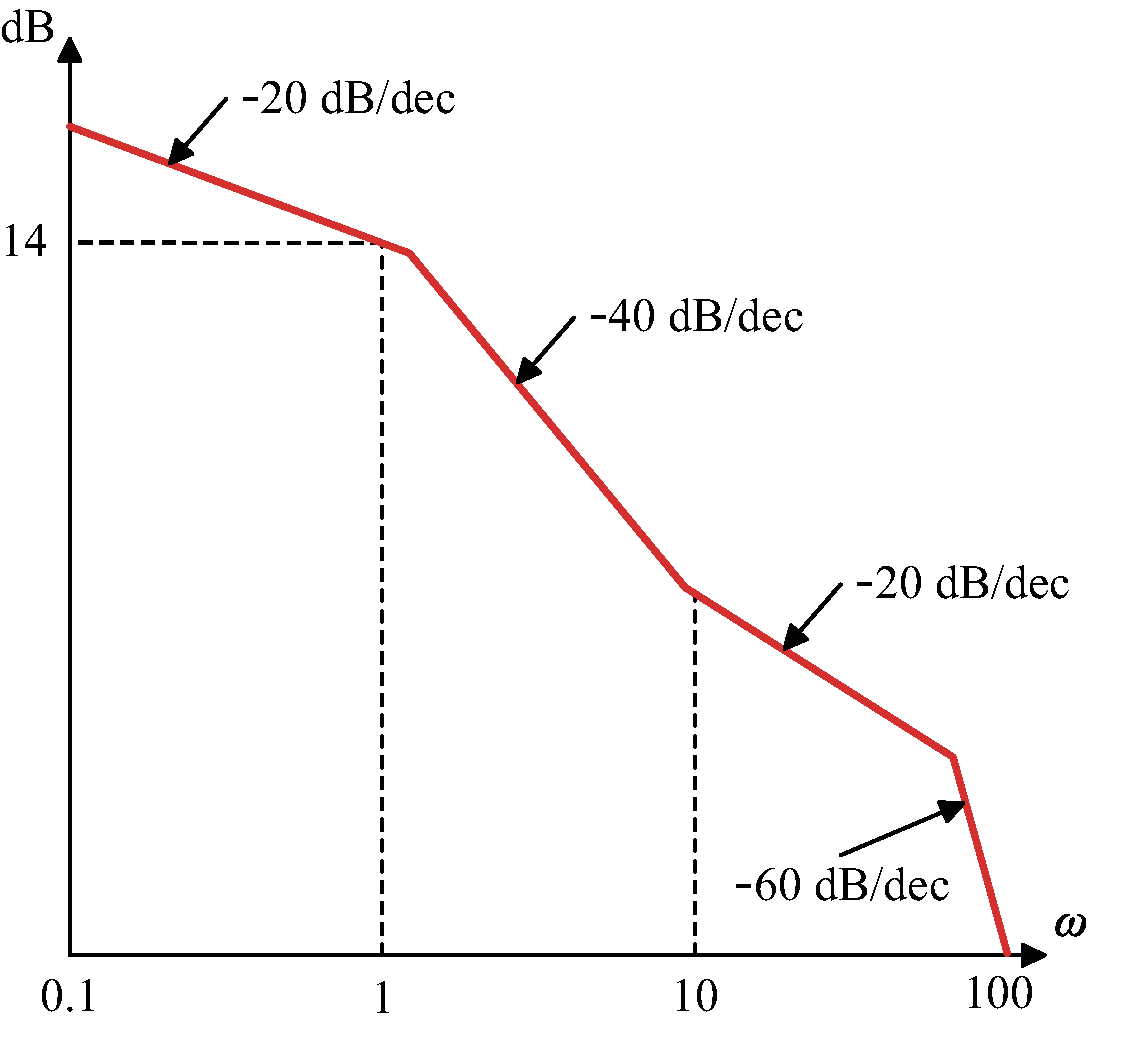
\includegraphics[width=0.45\linewidth]{pic/5.4.pdf}
	\caption{\ref{5.4}$\,$概略Bode图}
	\label{F5.4}
\end{figure}

用Matlab绘制出Bode图如图\ref{F5.4.2}.
\begin{figure}[!htb]
	\centering
	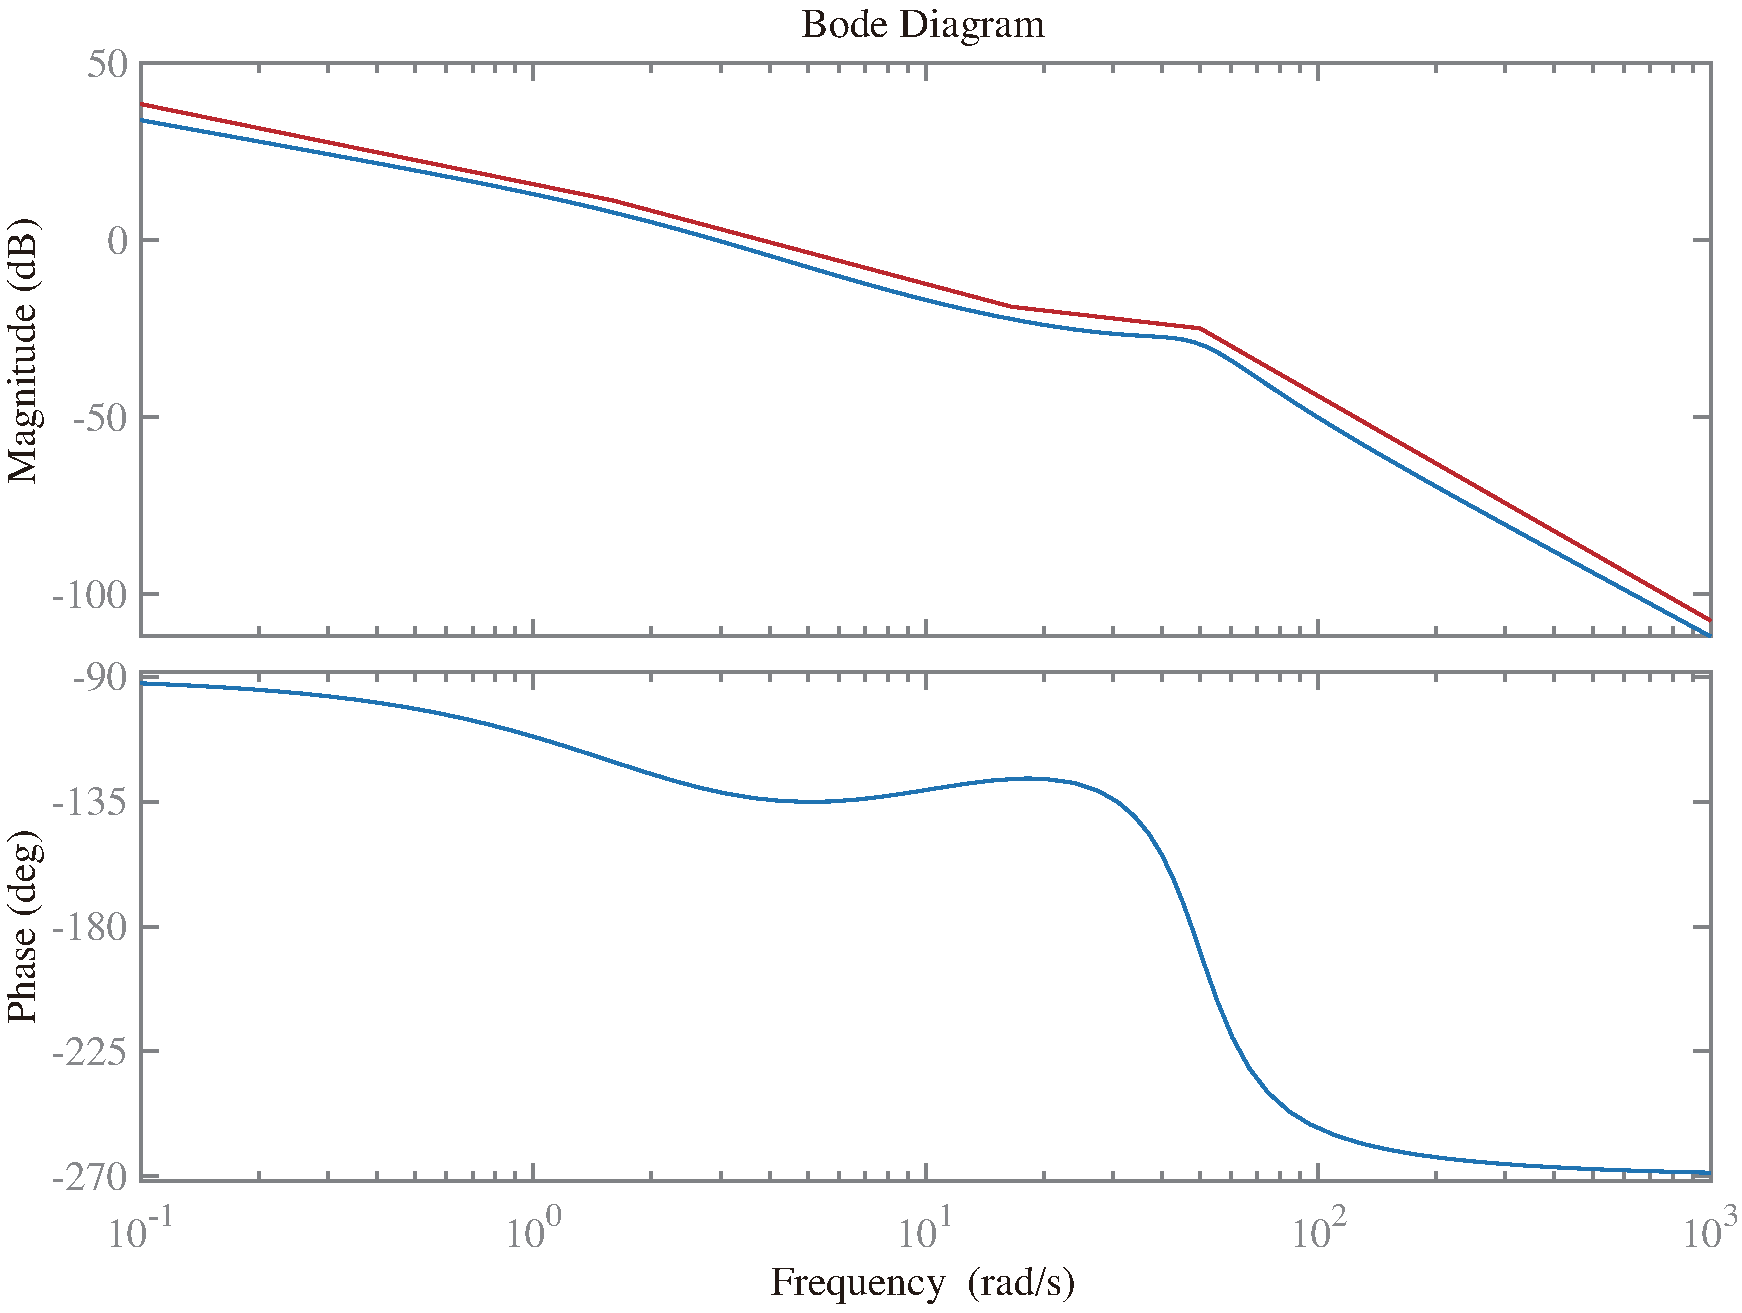
\includegraphics[width=0.7\linewidth]{pic/5.4.bode.pdf}
	\caption{\ref{5.4}$\,$实际Bode图}
	\label{F5.4.2}
\end{figure}
\warn[
\hspace*{2em}首先必须将传递函数写成标准形式!
]
\newpage

\vspace*{-2em}
\examples \label{5.5}一最小相位系统的Bode渐近幅频特性图如下:
\begin{figure}[!htb]
	\centering
	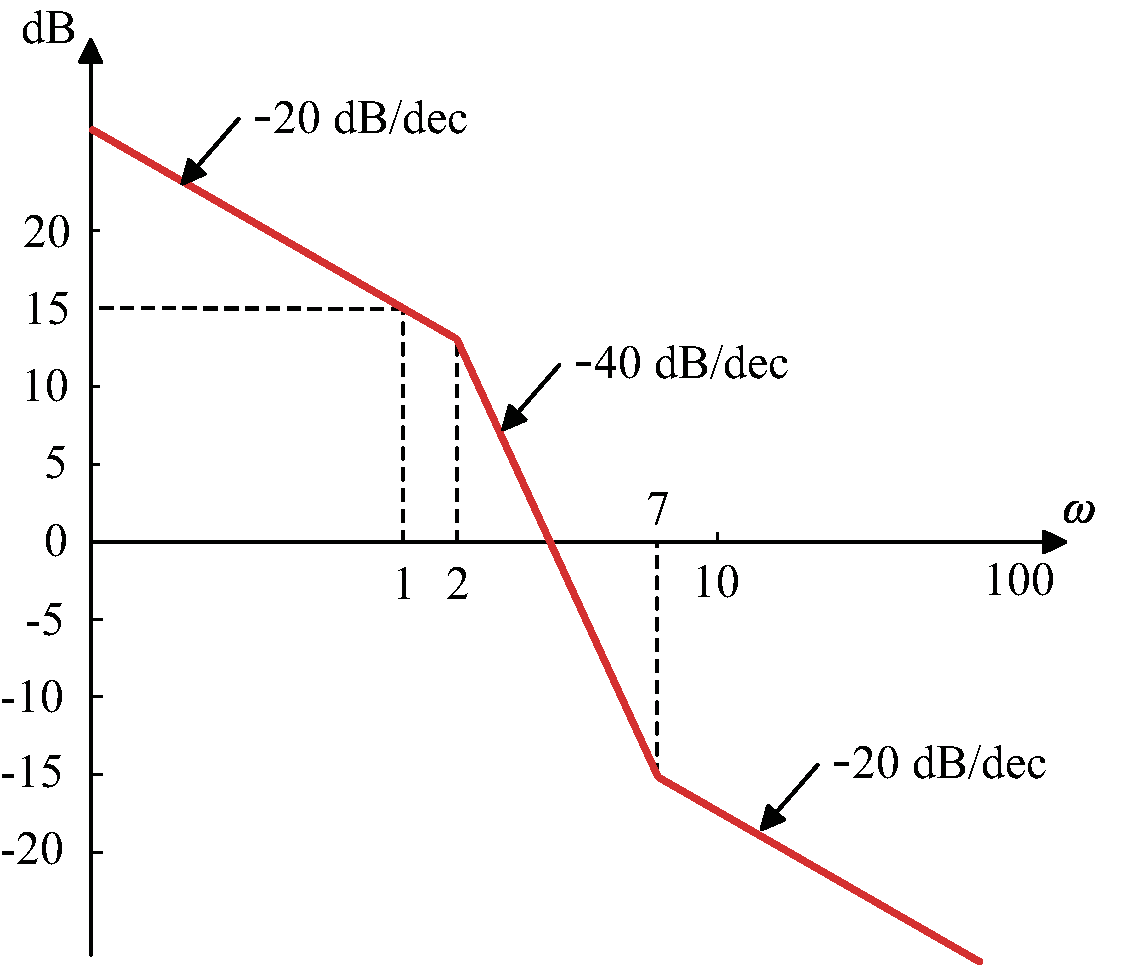
\includegraphics[width=0.45\linewidth]{pic/5.5.pdf}
	\caption{\ref{5.5}$\,$题图}
	\label{F5.5}
\end{figure}

确定其开环传递函数。

\solve 由图可以判断传递函数具有如下形式:
\begin{align*}
	G(s) = \dfrac{K(\tau s + 1)}{s(Ts + 1)}
\end{align*}
由图可以知道,斜率变化了两次
\begin{itemize}
	\item 开始时斜率为$-$20dB \quad $\Rightarrow$ \quad 对应积分环节
	\item $\omega = 2$时斜率$-20$dB \quad $\Rightarrow$ \quad 对应转折频率为$\omega = 2$的一阶环节,可以得到$T = \dfrac{1}{\omega} = \dfrac{1}{2}$.
	\item $\omega = 7$时斜率$+$20dB \quad $\Rightarrow$ \quad 对应转折频率为$\omega = 7$的一阶微分环节,可以得到$\tau = \dfrac{1}{\omega} = \dfrac{1}{7}$
\end{itemize}
又图线过点$(1, 15)$,此时渐近线仅积分环节不为0,所以
\begin{align*}
	\lg K - 20\lg 1 = 15 \quad \Rightarrow \quad \lg K = 15 \quad \Rightarrow \quad K \approx 5.6
\end{align*}
所以对应的开环传递函数为
\begin{align*}
	G(s) = \dfrac{5.6(s/7 + 1)}{s(s/5 + 1)}
\end{align*}
\vspace*{-2em}

\warn[
\textbf{\large 绘制Nyquist图和Bode图总结}
{
\begin{enumerate}[\hspace*{1em} 1. ]
	\item \textbf{Nyquist图:“三点一调”}
	\begin{enumerate}[\hspace*{1em}]
		\item \ding{172} 若存在积分(微分)环节,计算$\omega = 0$处的幅值和相角
		\item \ding{173} 计算$\omega = 0^+$处的幅值和相角
		\item \ding{174} 计算$\omega = +\infty$处的幅值和相角
		\item \ding{175} 根据相频函数$\varphi(\omega)$的单调性将三个点连接起来
		\begin{itemize}
			\item 若$\varphi(\omega)$单调递减,则顺时针转
			\item 若$\varphi(\omega)$单调递增,则逆时针转
		\end{itemize}
	\end{enumerate}
	
	\item  \textbf{Bode图:“分环节,逐叠加”}
	\begin{itemize}
		\item 幅频特性曲线
		\begin{enumerate}[\hspace*{1em}]
			\item \ding{172} 将开环传递函数拆成简单的单个环节
			\item \ding{173} 分别计算每个环节的转折频率和斜率
			\item \ding{174} 将各个环节的作用效果叠加即可
		\end{enumerate}
	
		\item 相频特性曲线
		\begin{enumerate}[\hspace*{1em}]
			\item \ding{172} 将相频函数$\varphi(\omega)$利用公式\eqref{arctan}将所有反正切函数合并成一个$\arctan f(\omega)$项
			\begin{align}
				\arctan A \pm \arctan B = \arctan \dfrac{A \pm B}{1 \mp AB}
				\label{arctan}
			\end{align}
			\item \ding{173} 利用$f(\omega)$的单调性和极值即可绘制概略曲线
		\end{enumerate}
	\end{itemize}
\end{enumerate}
}
]
\vspace*{-2em}

\section{频率稳定判据}
\vspace*{-0.5em}
\subsection{幅角原理}
\ttheorem[保形映射定理]
对$s$平面上任一不经过奇点的闭围线,$F$平面上也对应于一条闭围线。\index{BXYS@保形映射}

设$F(s)$是一个复变函数,在$s$平面熵任选一个复数$s$,通过函数$F(s)$的映射关系,可以在$F(s)$平面上找到响应的像。设
\begin{align}
	 F(s) = \dfrac{\displaystyle \prod_{i = 1}^{m}s - z_i}{\displaystyle \prod_{i=1}^{n} s- p_i}
\end{align}
设$s$沿着$\Gamma_s$移动时,$F(s)$相角变化为$\Delta \angle F(s) $,所以
\begin{align}
	\Delta \angle F(s) = \Delta \angle \left[\dfrac{\displaystyle \prod_{i = 1}^{m}s - z_i}{\displaystyle \prod_{i=1}^{n} s- p_i} \right]= \sum_{i = 1}^{m} \angle (s - z_i) - \sum_{j = 1}^{n} \angle (s - p_j)
\end{align}


\begin{figure}[!htb]
	\centering
	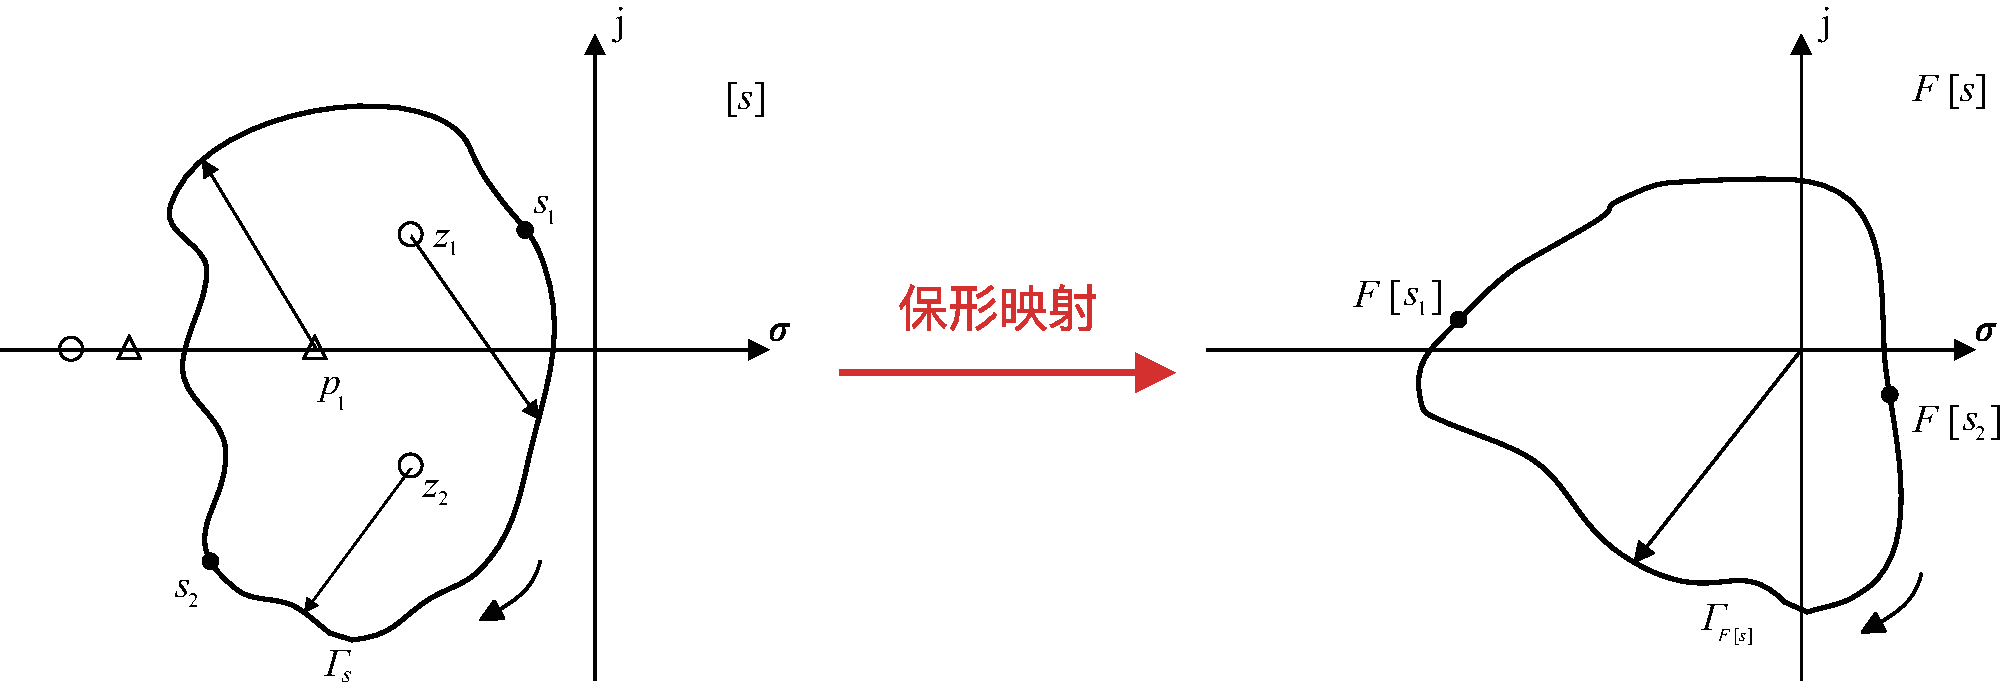
\includegraphics[width=0.85\linewidth]{pic/保形映射.pdf}
	\caption{保形映射}
	\label{保形映射}
\end{figure}

由图\ref{保形映射}可知,闭合路径$\Gamma_s$包围了两个零点$z_1,z_2$和一个极点$s_1$,其余零点和极点都分布在$\Gamma_s$以外。因此,当$s$沿闭合路径$\Gamma_s$顺时针移动一周时,由于只有$s$和闭合路径包围内的零点、极点构成的向量顺时针旋转了一周,其余向量角度没有变化。所以$\angle (s - z_1) = -2\pi, \angle (s - z_2) = -2 \pi, \angle (s - p_1) = -2 \pi$(规定逆时针方向为正),即
\[\Delta \angle F(s) = \angle (s - z_1) + \angle (s - z_2) = -2 \pi - \angle (s - p_1) = - 2 \pi\]

说明$F(s)$绕曲线顺时针旋转了一圈。

\theorem[幅角原理]
如果闭轨线$\Gamma_s$内$F(s)$有$Z$个零点、$P$个$F(s)$的极点,则$s$依$\Gamma_s$顺时针转一圈时,在$F(s)$平面上,$F(s)$曲线\textbf{绕原点逆时针转}的圈数$N$为$P$和$Z$之差,即\index{FJYL@幅角原理}
\begin{align}
	N = P - Z
\end{align}

\subsection{Nyquist稳定判据}

\begin{figure}[!htb]
	\centering
	\begin{tikzpicture}[circuit ee IEC]
		\node(A) [draw, inner sep =6pt]{$G(s)$};
		\node(B) [draw, inner sep =6pt, below of = A, node distance = 1cm]{$H(s)$};
		\node[bulb] (O) [draw, inner sep =5pt, left of = A, node distance = 2cm, label = -95:$-$]{};
		
		\draw[arrows={-Stealth}](-3cm, 0) -- (O)node[near start, above = 0mm]{$R(s)$} -- (A) -- (2cm, 0cm)node[midway, above = 0mm,xshift = 5mm]{$C(s)$};
		\draw[arrows={-Stealth}](1.5cm, 0cm) -- +(0cm, -1cm) -- (B) -- (-2cm,-1cm) -- (O);
	\end{tikzpicture}
	\caption{典型反馈控制系统}
	\label{典型反馈控制系统}
\end{figure}

\begin{enumerate}[1.]
	\item \textbf{辅助函数}\\
	\hspace*{2em}Nyquist 稳定性判据是通过开环传递函数确定闭环稳定性的频率域方法。考虑如图\ref{典型反馈控制系统}所示的闭环系统:
	\begin{align}
		G(s) = \dfrac{N_1(s)}{D_1(s)}\\[0.5em]
		H(s) = \dfrac{N_2(s)}{D_2(s)}
	\end{align}
	由此可以得到开环传递函数和闭环传递函数
	\begin{align}
		G(s)H(s) &= \dfrac{N(s)}{D(s)}\\[0.5em]
		\varPhi(s) = \dfrac{G(s)}{1 + G(s)H(s)} &= \dfrac{D(s)}{D(s) + N(s)}\\[0.5em]
		D= D_1D_2,& \,\,N = N_1N_2\notag
	\end{align}

	\hspace*{2em}定义
	\begin{align}
		F(s) = 1 + G(s)H(s) = \dfrac{D(s) + N(s)}{D(s)}
	\end{align}
	为\dy[辅助函数]{FZHS}。对于一般的物理过程,开环传递函数分母的幂次比分子的幂次高,即
	\begin{align*}
		\deg(N) < \deg(D)
	\end{align*}
	从而可以得到它具有的几个特点:
	\begin{itemize}
		\item 分子是闭环特征方程,分母是开环特征方程。
		\item 零点和极点分别是闭环和开环的特征根。
		\item 零点的个数与极点的个数相同。
		\item $F(s)$与系统开环传递函数只差常数1。
	\end{itemize}
	\vspace*{1em}

			
\begin{figure}[!htb]
	\centering
	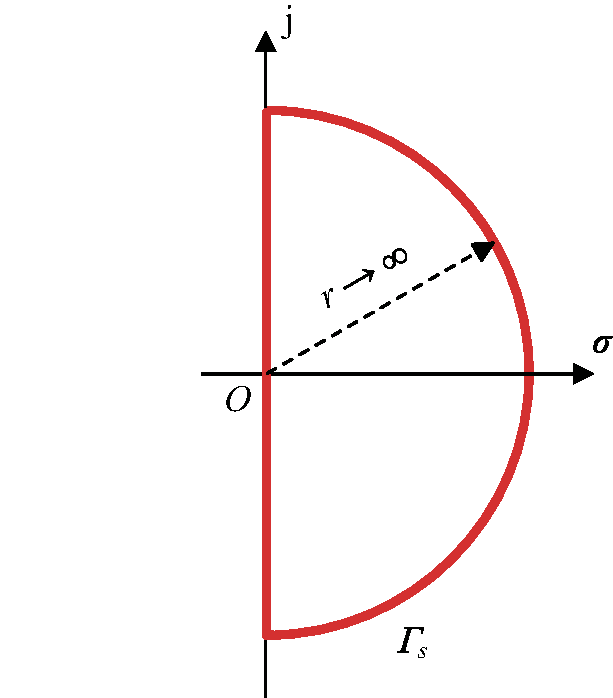
\includegraphics[width=0.3\linewidth]{pic/转圈数.pdf}
	\caption{N的确定}
	\label{转圈数}
\end{figure}

\item \textbf{Nyquist稳定判据}\\
	\hspace*{2em} 做如图\ref{转圈数}所示的闭环曲线$\varGamma_s$,对$F(s)$应用幅角原理,可以得到
	\begin{align}
		N = P - Z
	\end{align}
	其中,
	\begin{itemize}
		\item $P$\quad 不稳定开环极点的个数
		\begin{itemize}
			\item 可以直接由辅助函数得到。
		\end{itemize}
		\item $N$\quad $s$沿$\Gamma_s$顺时针转一圈时,$F(s)$逆时针包围原点的圈数
		\begin{itemize}
			\item 如图\ref{转圈数}. 由于
			\begin{align*}
				\lim\limits_{s \to \infty} F(s) = \lim\limits_{s \to \infty} \dfrac{D(s) + N(s)}{D(s)} = 0
			\end{align*}
			$s$沿半圆顺时针运动时, $F(s)$始终为0,即$F(s)$绕原点的圈数仅由$F(\j \omega), \,\, \omega : -\infty \to +\infty$确定。
			
		\end{itemize}
		\item $Z$\quad 不稳定闭环极点的个数
		\begin{itemize}
			\item $Z=0$ \quad 系统稳定。
			\item $Z>0$ \quad 系统不稳定且不稳定闭环极点的个数为$Z$。
		\end{itemize}
	\end{itemize}
	
\item \textbf{Nyquist稳定判据的简化}
	\begin{enumerate}[(1) ]
		\item 辅助函数$F(s) = 1 + G(s)H(s)$绕$(0,\j 0)$逆时针旋转的圈数$\Longleftrightarrow$开环传递函数$G(s)H(s)$绕$(-1,\j 0)$逆时针旋转的圈数。
		
		\item 如图\ref{转圈数}.由于$s\to \infty, G(s)H(s) \to 0$,所以$s$沿半圆顺时针运动时,$G(s)H(s)$始终为0。\\
		令$s = j \omega $,则$G(\j \omega )H(\j \omega)$绕$(-1,\j 0)$的圈数仅由$G(\j \omega)H(\j \omega), \,\, \omega : -\infty \to +\infty$确定。
		
		\item 由于$G(\j \omega)H(\j \omega)$与$G(- \j \omega) H(- \j \omega)$的取值对称,且点$(-1, \j 0)$位于实轴上,所以只需要确定$\omega : 0 \to +\infty $ 时,开环幅频特性曲线绕$(-1, \j 0)$点的圈数,再乘以2即可。
	\end{enumerate}

	\theorem[Nyquist稳定判据]
	一个LTI系统是稳定的充要条件是
	\begin{align}
	Z = P - 2 N = 0
	\end{align}
	\vspace*{-3.5em}
	
	其中,\vspace*{-0.5em}
	\begin{enumerate}[\hspace*{2em}]
		\item $P$\quad 不稳定开环极点的个数:可以直接由开环传递函数得到。
	
		\item $N$\quad $\omega : 0 \to \infty$时,开环幅相特性$G(\j \omega)H(\j \omega)$曲线绕点$(-1, \j 0)$逆时针旋转的圈数
		
		\item $Z$\quad 不稳定闭环极点的个数
	\end{enumerate}
	
	\examples \label{5.6}单位负反馈系统的开环传递函数如下:
	\begin{align*}
		G(s) = \dfrac{K}{(T_1s+1)(T_2s+1)(T_3s+1)}, \quad T_i > 0, K>0
	\end{align*}
	讨论其稳定性。
	\vspace*{-0.5em}
	
	\solve 由开环传递函数知,开环极点的个数为0,即$P=0$,绘制三种情况的幅相概略图如图\ref{F5.6}.
	
	\begin{figure}[!htb]
		\centering
		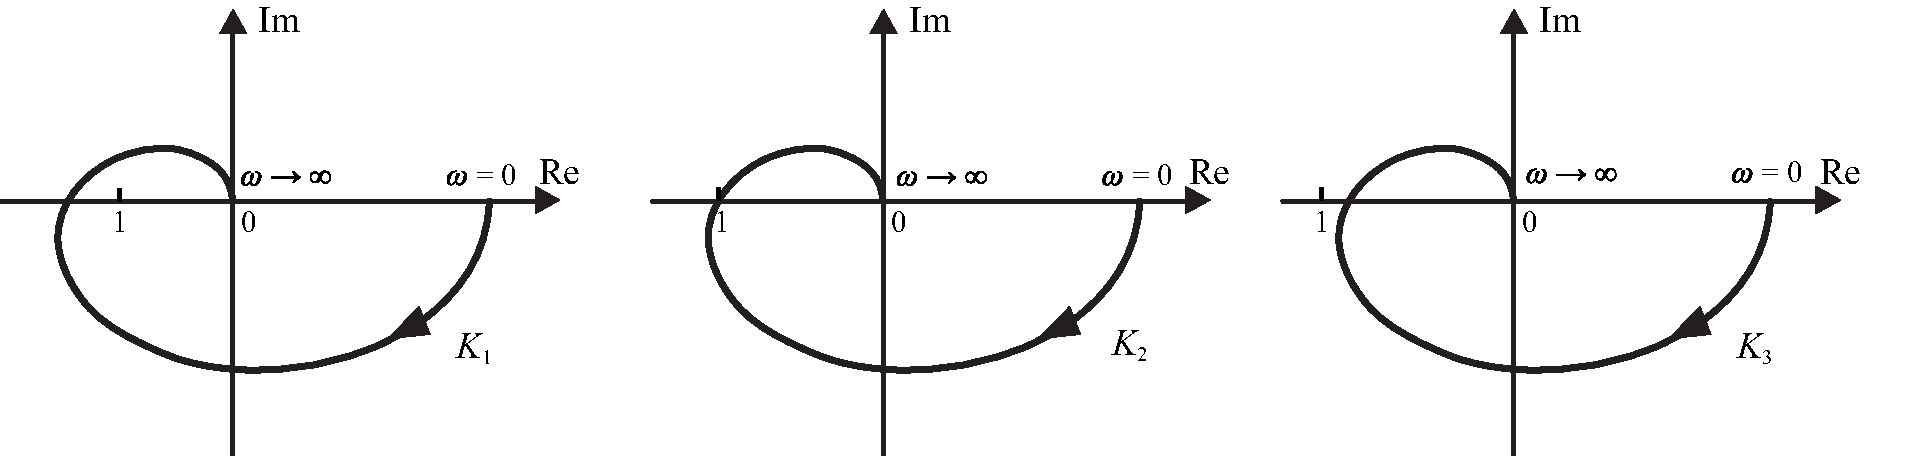
\includegraphics[width=0.9\linewidth]{pic/5.6.pdf}
		\caption{\ref{5.6}解图}
		\label{F5.6}
	\end{figure}
\end{enumerate}

\subsection{对数频率稳定性判据}
考虑单位负反馈系统的开环传递函数如下:
\begin{align*}
	G(s) = \dfrac{K}{(T_1s+1)(T_2s+1)(T_3s+1)}, \quad T_i > 0, K>0
\end{align*}
这里,假设$P=0,N=-1$,系统不稳定,如图\ref{F5.6}中的左边第一个图。关键是在穿越负实轴时$|A|>1$.对应的Bode图如图\ref{对数稳定}.
\begin{figure}[!htb]
	\centering
	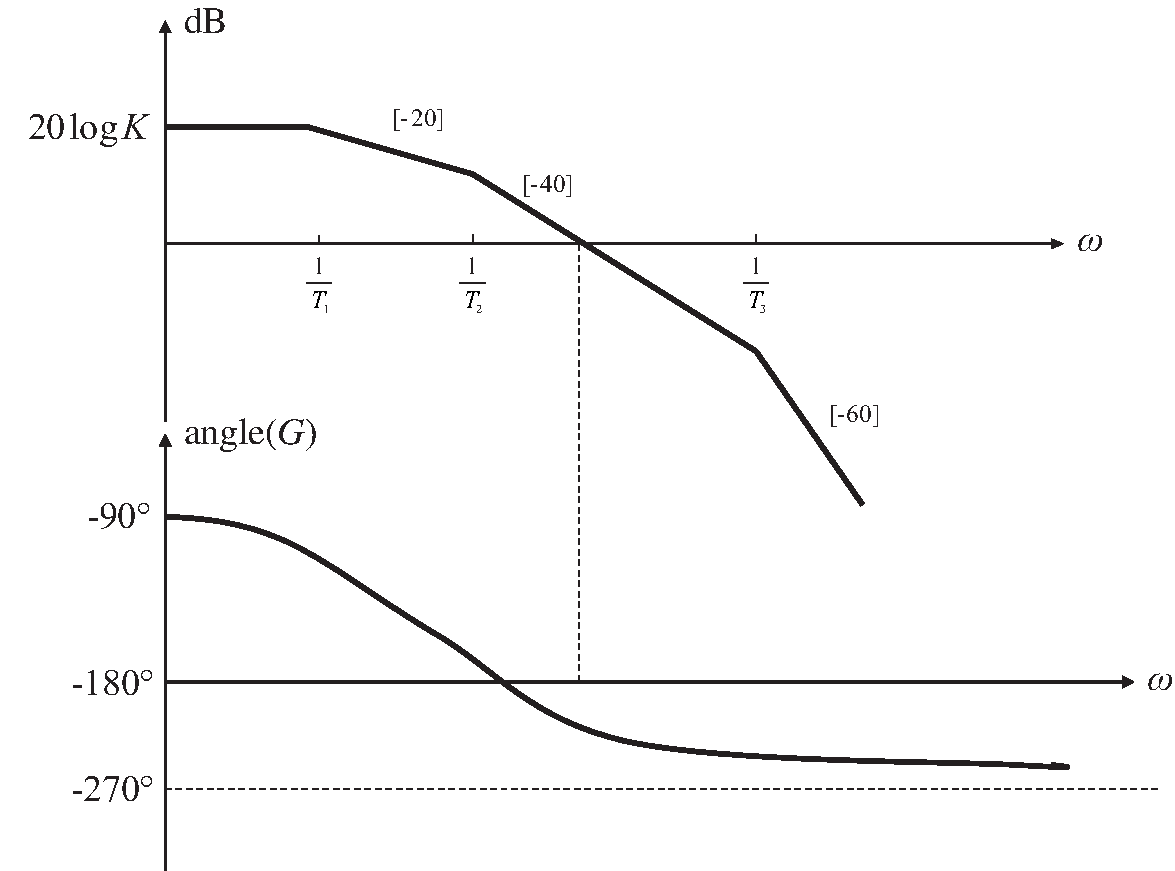
\includegraphics[width=0.7\linewidth]{pic/对数判据.pdf}
	\caption{对数频率稳定判据}
	\label{对数稳定}
\end{figure}

\theorem[对数频率稳定判据]
一个LTI系统稳定,当且仅当由
\begin{align}
	N_+  - N_- = \dfrac{P - Z}{2}
\end{align}
其中
\vspace*{-0.5em}
\begin{enumerate}[\hspace*{2em}]
	\item $P$\quad 不稳定开环极点的个数:可以直接由开环传递函数得到。\vspace*{-0.5em}
	
	\item $N_+$\quad 在$L(\omega_i) = 20\lg\big(A(\omega_i)\big) > 0$时,$\angle G$正穿越
	\footnote{正穿越:相频特性曲线由下向上穿越$-180\degree$线一次,称为一次正穿越;对于相频曲线从$-180\degree$线开始向上的情况,称为半次正穿越,负穿越同理,只是方向改为由上向下穿越$-180\degree$线。}
	$-180\degree$线的次数;\vspace*{-0.5em}
	
	\item $N_-$\quad 在$L(\omega_i) = 20\lg(A\big(\omega_i)\big) > 0$时,$\angle G$负穿越$-180\degree$线的次数;\vspace*{-0.5em}
	
	\item $Z$\quad 不稳定闭环极点的个数
	
\end{enumerate}

\subsection{开环含积分环节时的稳定性判据}
考虑如下开环传递函数:
\begin{align}
	G(s)H(s) = \dfrac{K}{s(Ts + 1)}
\end{align}
这里,$s$是一个奇点,故Nyquist闭围线$\varGamma_s$必须修改:

考虑如下半径$\varepsilon > 0$无限小的四分之一圆弧:
\begin{align}
	s = \varepsilon \e^{\j \theta}
\end{align}
其中,当$\omega$由0变化到$0^+$时,$\theta$从$0\degree$转过$90\degree$。如图\ref{积分环节的幅相特性}.
\begin{figure}[!htb]
	\centering
	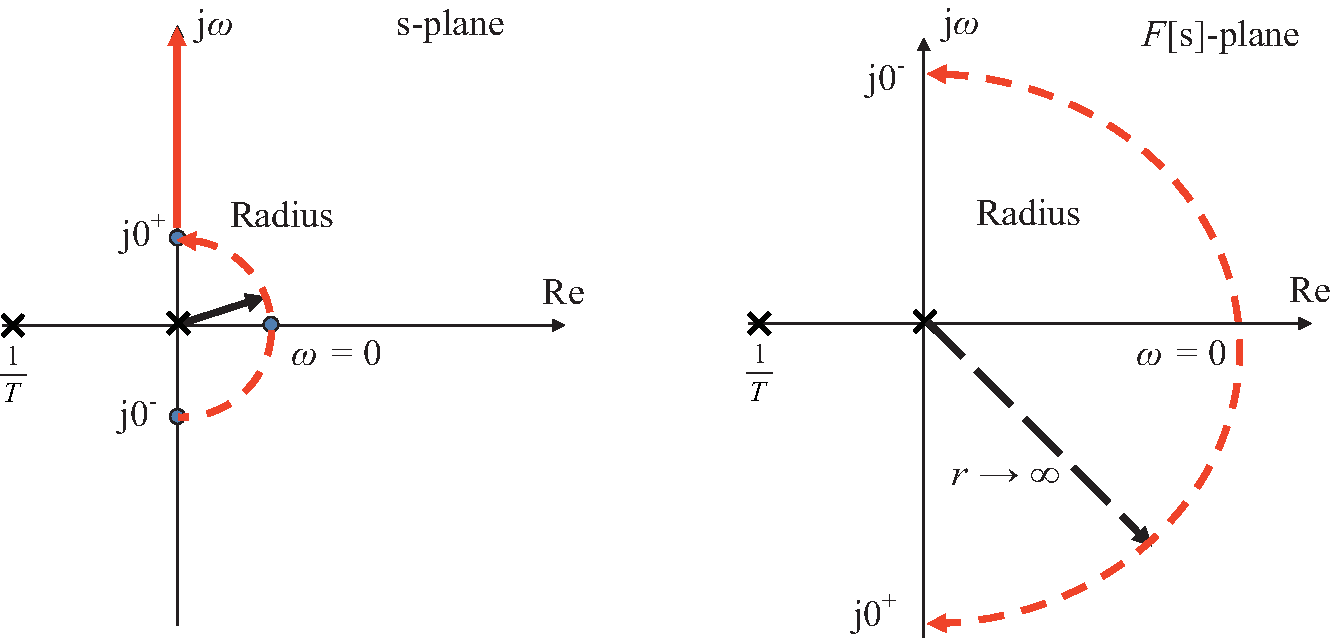
\includegraphics[width=0.7\linewidth]{pic/积分环节幅相特性.pdf}
	\caption{积分环节的幅相特性}
	\label{积分环节的幅相特性}
\end{figure}

因此,$\dfrac{1}{s}$被视为稳定极点。对含有积分$\dfrac{1}{s}$的被控对象,
\begin{align}
	\dfrac{1}{s} = \dfrac{1}{\varepsilon} \cdot \e^{- \j \theta}, \quad \theta : 0 \to -90\degree
\end{align}

\noindent 为了简化问题,我们仅考虑$\omega \ge 0$的情形,
\begin{itemize}
	\item 首先计算$\omega = 0$,这时积分环节的角度为0,其余环节仍然按$\omega = 0$计算。\vspace*{-0.5em}
	\item 再计算$\omega = 0^+$积分环节的角度为$-90\degree$,其余环节也仍然按$\omega = 0^+$计算。
\end{itemize}
对于考虑的开环传递函数的相频特性函数$\varphi(\omega) = -\arctan\dfrac{\omega}{0} - \arctan(T\omega)$
\begin{align*}
	\begin{cases}
		\, \omega = 0 \Rightarrow & \varphi(0) = 0 - 0 = 0\\
		\, \omega = 0^+ \Rightarrow & (0^+) = -90\degree = -90\degree
	\end{cases}
\end{align*}

所以$\omega \le 0$的根轨迹如图\ref{积分环节的幅相特性2}.
\begin{figure}[!htb]
	\centering
	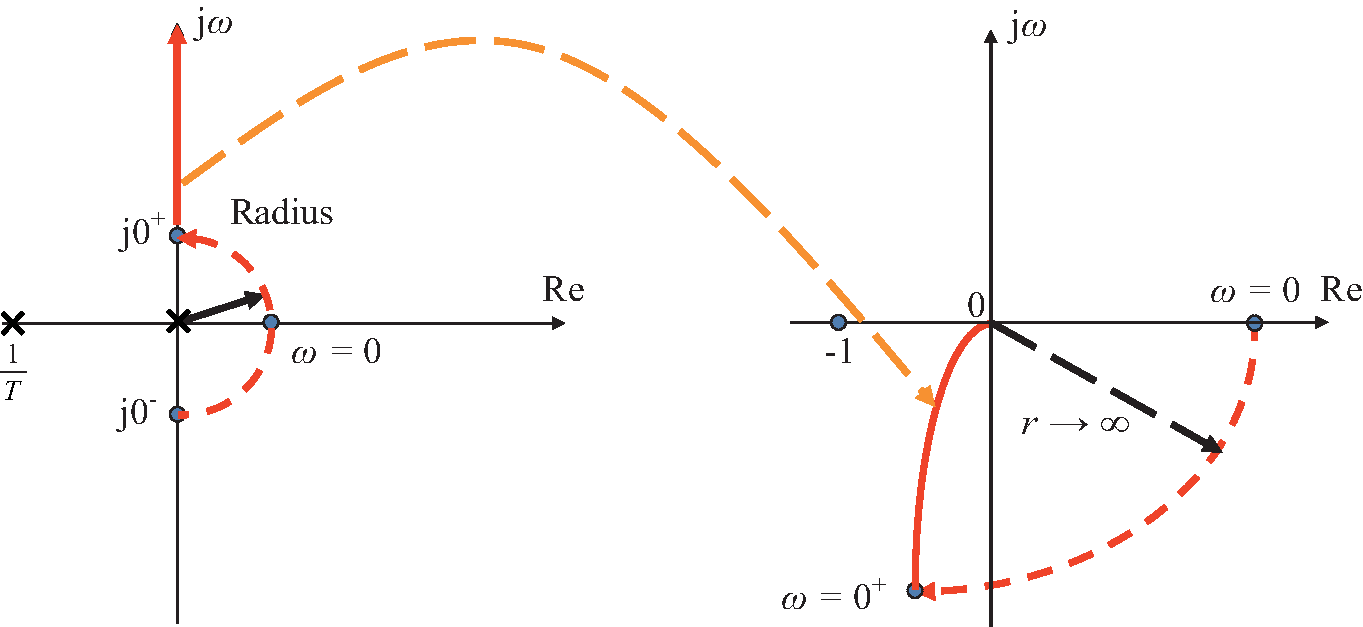
\includegraphics[width=0.7\linewidth]{pic/积分环节幅相特性2.pdf}
	\caption{积分环节的幅相特性2}
	\label{积分环节的幅相特性2}
\end{figure}

\vspace*{-3em}
\examples \label{5.7}已知某个系统的开环传递函数如下
\begin{align*}
	G(s)H(s) = \dfrac{K}{s(Ts - 1)}, \quad T>0,\,\, K>0
\end{align*}
利用Nyquist判据判断系统的稳定性。

\solve  系统的相频特性函数为
\begin{align*}
	\varphi(\omega) = \angle\big[G(s)H(s)\big] &= - \text{sign}(\omega)\cdot 90\degree -\arctan(-T\omega) \\
	&= - \text{sign}(\omega) \cdot 90\degree -\big[180\degree - \arctan(T\omega)\big]
\end{align*}

当$\omega = 0$时,
\[
	\varphi(0) =  -180 - 0 \cdot 90 \degree + 0\degree = -180 \degree
\]

当$\omega = 0^+$时,
\[\varphi(0^+) = -180\degree - 1 \cdot 90 \degree + 0\degree  = -270 \degree\]

当$\omega \to +\infty$时,
\[
	\varphi(+\infty) = -180\degree - 1 \cdot 90 \degree + 90\degree  = -180 \degree
\]

由于$P = 1$,其幅相特性曲线图如图\ref{F5.7}.由图可知,$N = -\dfrac{1}{2}$,由Nyquist判据可知
\[
Z = P - 2N = 2 > 0
\]
所以系统是不稳定的。
\begin{figure}[!htb]
	\centering
	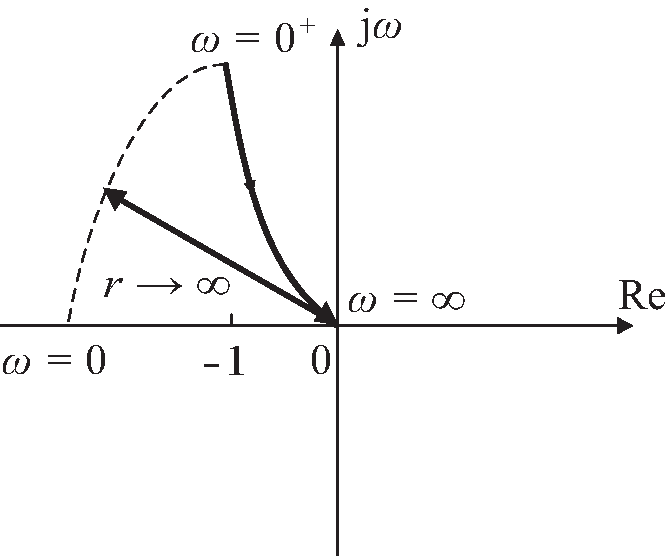
\includegraphics[width=0.3\linewidth]{pic/5.7.pdf}
	\vspace*{-1em}
	\caption{\ref{5.7}$\,$幅相特性曲线图}
	\label{F5.7}
\end{figure}
\vspace*{-0.5em}
\subsection{条件稳定性}
\vspace*{-0.5em}
如图\ref{条件稳定性}所示,当开环增益增加或减小时,系统都会变得不稳定,这样的系统称为\dy[条件稳定系统]{TJWDXT}。
\begin{figure}[!htb]
	\centering
	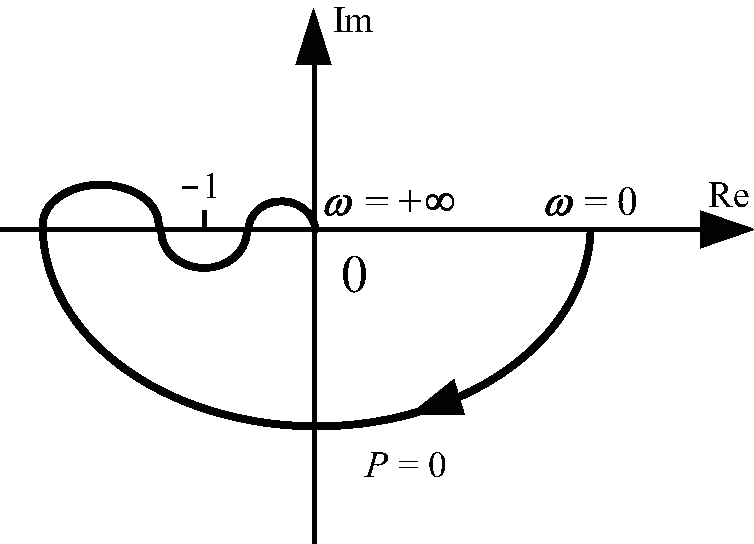
\includegraphics[width=0.4\linewidth]{pic/条件稳定性.pdf}
	\vspace*{-1em}
	\caption{条件稳定性}
	\label{条件稳定性}
\end{figure}

\subsection{稳定裕度}
\noindent \textbf{1. 稳定裕度概念}

两个系统的开环幅相特性曲线表明,极点离虚轴越近,则幅相特性曲线就离$(-1, \j0)$点越近。

通常,用接近$G(\j \omega)$幅相特性曲线$-1$点的程度来衡量系统的\dy[稳定裕度]{WDYD},如图\ref{稳定裕度1}.
\begin{figure}[!htb]
	\centering
	\begin{minipage}{0.4\linewidth}
		\centering
		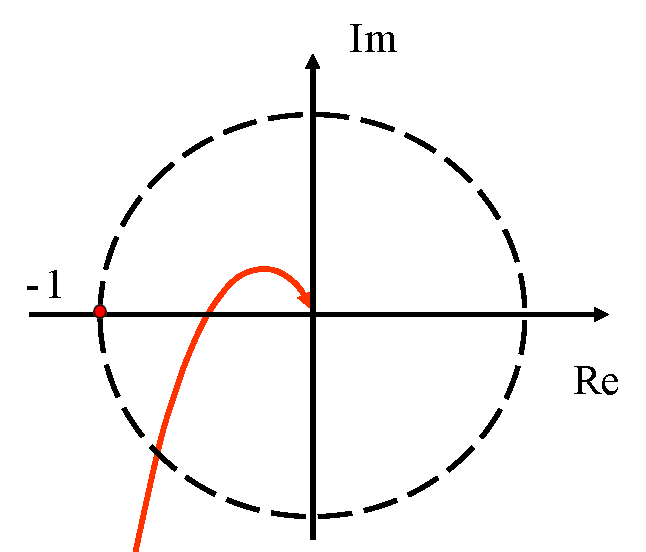
\includegraphics[width=0.9\linewidth]{pic/稳定裕度1.pdf}
	\end{minipage}
	\begin{minipage}{0.4\linewidth}
		\centering
		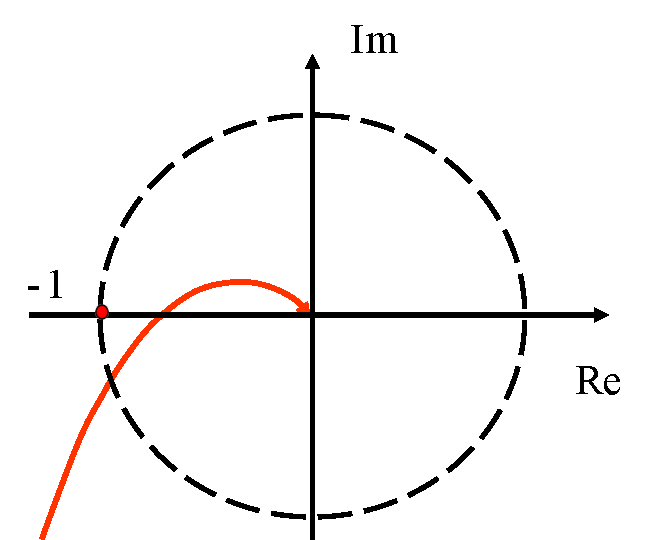
\includegraphics[width=0.9\linewidth]{pic/稳定裕度2.pdf}
	\end{minipage}
	\caption{稳定裕度示意图}
	\label{稳定裕度1}
\end{figure}

\noindent \textbf{2. 模稳定裕度与相稳定裕度}
\begin{figure}[!htb]
	\begin{minipage}{0.4\linewidth}
		\centering
		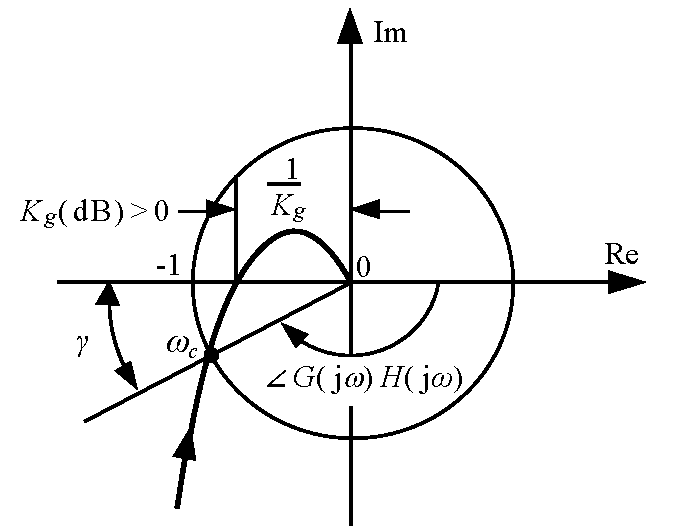
\includegraphics[width=\linewidth]{pic/稳定裕度3.pdf}
	\end{minipage}
	\begin{minipage}{0.6\linewidth}
	\centering
	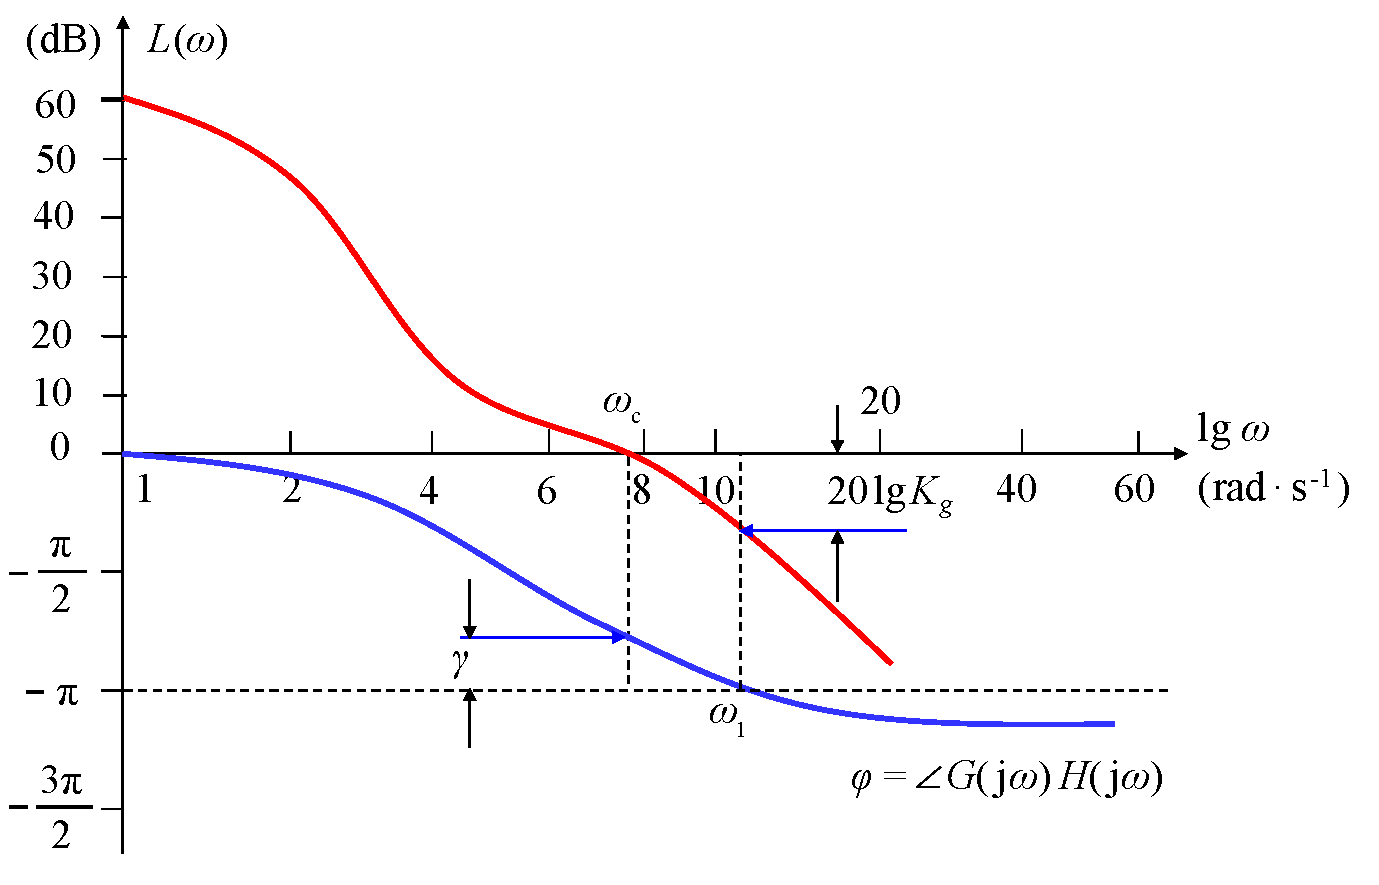
\includegraphics[width=\linewidth]{pic/稳定裕度4.pdf}
	\end{minipage}
	\caption{稳定裕度在Nyquist图和Bode图上的定义}
	\label{稳定裕度2}
\end{figure}
\vspace*{-1em}
\begin{itemize}
	\item \dy[相稳定裕度]{XWGYD}
	\begin{align}
		\gamma = 180 \degree + \angle G(\j \omega_{\text{c}})H(\j \omega_{\text{c}}) = 180 \degree + \varphi(\omega_{\text{c}})
	\end{align}
	其中,$\omega_{\text{c}}$称为\dy[截止频率]{JZPL},满足$|G(\j \omega_{\text{c}})H(\j \omega_{\text{c}})| = A(\omega_{\text{c}}) = 1$.
	
	\item \dy[模稳定裕度]{MWDYD}
	\begin{align}
		K_g = \dfrac{1}{|G(\j \omega_1)H(\j \omega_1)|} = \dfrac{1}{A(\omega_1)}\\[0.5em]
		K_g(\text{dB}) = 20 \lg K_g = -20 \lg A(\omega_1)
	\end{align}
	其中,$\omega_{\text{1}}$称为\dy[交接频率]{JJPL},满足$\angle G(\j \omega_1)H(\j \omega_1) = \angle \varphi(\omega_1) = - 180 \degree$.
\end{itemize}
\vspace*{-2.5em}
\warn[
关于相稳定裕度和模稳定裕度
{
\begin{enumerate}
	\item 相稳定裕度和模稳定裕度均是基于\textcolor{red}{开环}幅频和相频曲线,用于衡量系统对$-1$点的接近程度,是重要的设计指标。
	\item 两个指标需同时使用。单独采用相稳定裕度或模稳定裕度均不足以描述系统对$-1$点的接近程度。
	\item \textcolor{red}{对最小相位系统,系统稳定,$\gamma, K_g$一定为正;负的稳定裕度表明系统不稳定。}
	\item 合适地选取$\gamma, K_g$可保证系统对于建模误差和元部件参数变化等的鲁棒性,以及在在谐振频率附近的闭环性能。一般地,若$30\degree \le \gamma \le 60\degree$及$K_g \ge 6$dB,则对最小相位系统而言,闭环系统将具有较好的鲁棒性。
	\item 条件稳定系统可能具有几个交接频率;某些高阶系统可能具有不止一个的截止频率。若一个稳定系统有不止一个截止频率,要用\textcolor{red}{最大的截止频率求相稳定裕度}。
\end{enumerate}
}
]

\examples 确定下列开环传递函数的相和模稳定裕度
\[
G(s) = \dfrac{2}{s(s + 1)(0.2s + 1)}
\]
\vspace*{-3em}

\solve 由稳定裕度的定义
\vspace*{1em}

\noindent
\begin{inparaitem}
	\item 相稳定裕度
	\[
		|A(\omega_{\text{c}})| = 1 \quad \Rightarrow \quad \omega_{\text{c}} = 1.2247
	\]
	\vspace*{-2em}
	\[
		\varphi(\omega_{\text{c}}) = - 90 \degree - \arctan \omega_{\text{c}} - \arctan \dfrac{\omega_{\text{c}}}{5}= -154.53 \degree
	\]
	\vspace*{-2em}
	\[
		\gamma = 180 \degree + \varphi_{\text{c}} = 180 \degree - 154.53 \degree = 25.47 \degree
	\]
	\item 模稳定裕度
	\[
		\varphi(\omega_1) = - 90 \degree - \arctan \omega_1 - \arctan \dfrac{\omega_1}{5}= -180 \degree \quad \Rightarrow \quad \omega_1 \cdot \dfrac{\omega_1}{5} = 1 \quad \Rightarrow \quad \omega_1 = \sqrt{5}
	\]
	\vspace*{-2em}
	\[
		K_g = -20 \lg A(\omega_1) = -20 \lg \dfrac{1}{\omega_1 \cdot \sqrt{\omega_1^2 + 1} \cdot \sqrt{0.04\omega_1^2 + 1}} = - 20 \lg \dfrac{1}{6} = 20 \lg 6 = 9.54\, \text{dB}
	\]
\end{inparaitem}

\clearpage

\section{系统闭环频率特性与阶跃响应的关系}
\subsection{二阶系统阶跃响应与频率响应之间的关系}
考虑二阶系统欠阻尼的情况:$0<\zeta<1$
\begin{figure}[!htb]
	\centering
	\begin{tikzpicture}[circuit ee IEC,node distance=1.2cm]
		\node[bulb] (A)  [draw, inner sep=5pt,label=-80:$-$] {};
		\node (B) [draw, inner sep =4pt,right of = A, node distance = 2cm]{$\,\dfrac{\omega_\n^2}{s^2 + 2 \zeta \omega_\n s}\,$};
		
		\draw[arrows={-Stealth}] (-1cm,0cm) -- (A)node[near start, above = 0cm]{$R(s)$};
		\draw [arrows={-Stealth}] (A) -- (B);
		\draw[arrows={-Stealth}] (B) -- (4cm,0cm)node[near end, above =0cm]{$C(s)$};
		\draw[arrows={-Stealth}] (3.5cm,0cm) -- +(0cm, -1cm) -- (0cm,-1cm) -- (A);
	\end{tikzpicture}
	\caption{二阶系统结构图}
	\label{二阶系统结构}
\end{figure}

\noindent \textbf{1. 时域与频域}
\begin{itemize}
	\item 时域\\
	由\pageref{欠阻尼二阶公式}页的公式\eqref{欠阻尼二阶公式},可以得到
	\[
		h(t) = 1 - \dfrac{\e^{-\zeta \omega_\n t}}{\sqrt{1 - \zeta^2}}\sin (\omega_\text{d}t + \beta), \quad \quad \omega_{\text{d}} = \omega_{\n} \sqrt{1 - \zeta^2},\quad \beta = \arctan\left(\dfrac{\sqrt{1 - \zeta^2}}{\zeta}\right) = \arccos\zeta
	\]
	其超调量为
	\[
	\sigma \, \%  =\e^{- \pi \zeta / \sqrt{ 1 - \zeta^2}} \times 100 \%
	\]
	当$\zeta < 0.4$时,系统的超调量很大。
	
	\item 频域\\
	二阶系统的开环传递函数
	\[
	G(s) = \dfrac{\omega_\n^2}{s^2 + 2 \zeta \omega_\n s}
	\]
	由第\pageref{谐振峰值}页的公式\eqref{谐振频率},\eqref{谐振峰值}可得谐振频率和谐振峰值分别为
	\[
		\omega_r = \omega_\n \sqrt{1 - 2\zeta^2},\quad 
		M_r = \dfrac{1}{2 \zeta \sqrt{1 - \zeta^2}}\quad \quad 0< \zeta < \dfrac{\sqrt{2}}{2}
	\]
	其相稳定裕度为
	\begin{align}
		\gamma = 180\degree + \angle G(\j \omega_{\text{c}}) = \arctan \dfrac{2 \zeta}{\sqrt{\sqrt{4 \zeta^4 + 1}-2 \zeta^2}}
	\end{align}
\end{itemize}

\noindent \textbf{2. 时域指标和频域指标的关系}
\begin{itemize}
	\item 相稳定裕度$\gamma$与阻尼比$\zeta$\\
	\hspace*{2em} $\gamma,\zeta$在$0<\zeta < 0.6$近似为线性关系
	\begin{align}
		\zeta = \dfrac{\gamma}{100}
		\label{gz关系}
	\end{align} 
	特别地,对高阶系统,公式\eqref{gz关系}可用来估算系统的阻尼比。
	
	\item 谐振频率$\omega_r$和阻尼振荡角频率$\omega_{\text{d}}$
	\[
	\begin{cases}
		\, \omega_{\text{d}} = \omega_{\n} \sqrt{1 - \zeta^2}\\
		\, \omega_r = \omega_\n \sqrt{1 - 2\zeta^2}, \quad 0 < \zeta < 0.707
	\end{cases}
	\]
	 所以,当$\zeta $较小时,
	 \vspace*{-1em}
	 \begin{align}
	 	\omega_r \approx \omega_{\text{d}}
	 \end{align}
 
 	\item 谐振峰值$M_r$和超调量$\sigma\, \%$
 	\begin{align*}
 		\begin{cases}
 			\sigma \, \% =  =\e^{- \pi \zeta / \sqrt{1 - \zeta^2}} \times 100 \%\\
 			M_r = \dfrac{1}{2 \zeta \sqrt{1 - \zeta^2}}\quad \quad 0< \zeta < 0.707
 		\end{cases}
 	\end{align*}
 	$\zeta$ 越小,$M_r, \sigma \, \%$就越大。且若$\zeta >0.707$,无谐振峰;但在$0<\zeta <1$,振荡始终存在。
\end{itemize}
\vspace{0.5em}

\subsection{利用闭环幅频特性分析和估算系统的性能}
\vspace*{-1.5em}
\begin{figure}[!htb]
	\centering
	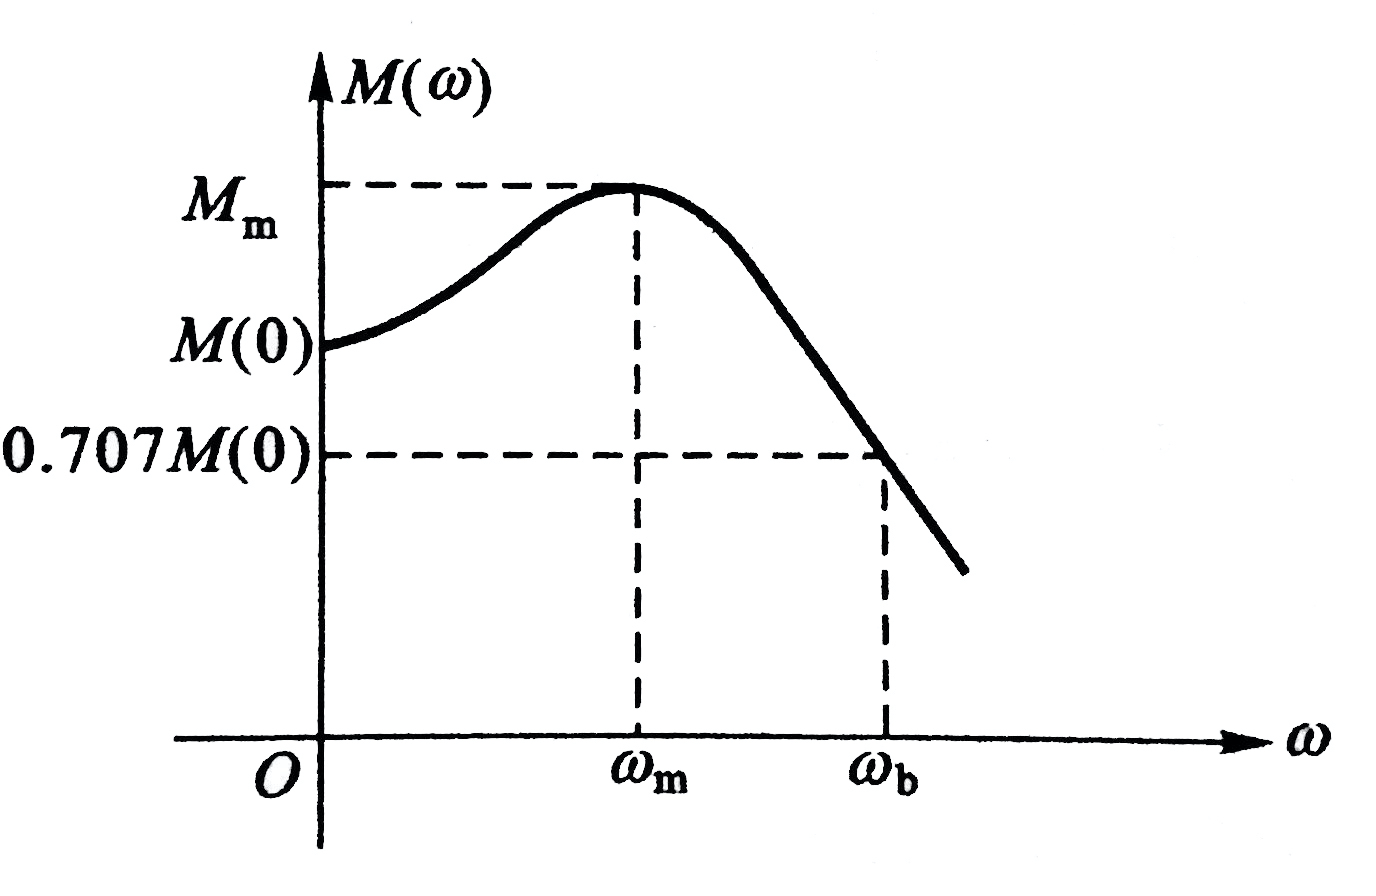
\includegraphics[width=0.4\linewidth]{pic/闭环幅频特性.jpeg}
	\vspace*{-2em}
	\caption{闭环幅频特性概略曲线}
	\vspace*{-1em}
	\label{闭环幅频特性}
\end{figure}
\begin{enumerate}[1. ]
		\item \dy[谐振峰值$M_m$]{XZFZ}
			\begin{itemize}
				\item 定义 \quad 幅频特性$M(\omega)$
				\footnote[1]{开环系统的幅频函数用$A(\omega)$表示,而闭环的幅频函数用$M(\omega)$表示。}的最大值。
				\item 作用 \quad 反映系统的平稳性。
				\begin{itemize}
					\item $M_m$大,说明系统的阻尼弱,动态过程的超调量大,平稳性差。
					\item $M_m$小,系统的平稳性好。
				\end{itemize}
				\item 应用 \quad 对具有一对闭环主导复极点的高阶系统,$M_r$ 可用于衡量相对稳定性:
				\begin{itemize}
					\item 良好的过渡过程应满足$1.0<Mr<1.4\quad (0$dB$<Mr<3$dB$, \,0.4 <\zeta < 0.7)$;
					\item 若$M_r>1.5$,系统响应将具有很大的超调。
				\end{itemize}
			\end{itemize}
		
		\item \dy[零频幅值$M(0)$]{LPFZ}
			\begin{itemize}
				\item 定义 \quad 零频率$\omega = 0$时的幅频值。
				\item 作用 \quad 反映系统的稳态误差(静差)。
				\begin{itemize}
					\item $M(0) = 1$,说明系统无稳态误差,即$e_{\text{ss}} = 0$。
					\item $M(0) \neq 1$,说明系统存在稳态误差,即$e_{\text{ss}} \neq 0$。
				\end{itemize}
			\end{itemize}
		
		\item \dy[带宽频率$\omega_{\text{b}}$]{DKPL}
		\begin{itemize}
			\item 定义 \quad $M(\omega)$的数值衰减到$0.707M(0)\,\,$(3dB)时所对应的频率。
			\item 作用 \quad 反映系统的快速性。
			\begin{itemize}
				\item $\omega_{\text{b}}$高,则曲线$M(\omega)$曲线由$M(0)\to 0.707 M(0)$所占据的区间$(0, \omega_{\text{b}})$较宽,表面系统复现快速变化的信号能力强,失真小。
			\end{itemize}
		\end{itemize}
		
		\item \textbf{频率尺度与时间尺度的反比性质}
				
			\theorem[相似定理]
			若两个闭环传递函数存在关系
			\vspace*{-1em}
			\begin{align}
				\varPhi_1(s) = \varPhi_2(n s) \quad \Rightarrow \quad \varPhi_1(\j \omega) = \varPhi_2(n \j \omega)
			\end{align}
			\vspace*{-3em}
			
			其中$n$为任意常数,则对应的单位阶跃响应具有如下关系
			\begin{align}
				h_1(t) = h_2 \left(\dfrac{t}{n}\right)
			\end{align}
			即系统的频率特性放宽$n$倍,对应的阶跃响应就快$n$倍。
				
				
				
		\item \textbf{抗高频干扰的能力}	\\
		\hspace*{2em} 闭环幅频$M(\omega)$在$\omega_{\text{b}}$处的斜率反映系统抗高频干扰的能力。
\end{enumerate}
\examples 求二阶系统的带宽频率$\omega_{\text{b}}$.

\solve 由闭环二阶系统的传递函数
\[
\varPhi(s) =  \dfrac{\omega_\n^2}{s^2 + 2 \zeta \omega_\n s + \omega_\n^2}
\]
得到
\[
M(\omega) = \dfrac{1}{\sqrt{ \big(1 - \omega^2 / \omega_{\text{n}}^2\big)^2+ 4 \zeta^2 \omega^2 / \omega_{\text{n}}^2}} 
\]
由于
\[
	M(0) = 1
\]
所以
\[
\dfrac{1}{\sqrt{ \big(1 - \omega_{\text{b}}^2 / \omega_{\text{n}}^2\big)^2+ 4 \zeta^2 \omega_{\text{b}}^2 / \omega_{\text{n}}^2}}  = \dfrac{1}{\sqrt{2}}M(0) = \dfrac{1}{\sqrt{2}}
\]
解得
\begin{align}
	\omega_{\text{b}} = \omega_{\n}\sqrt{\big(1 - \zeta^2\big) + \sqrt{\big(1 - \zeta^2\big)^2 + 1}}
\end{align}

\section{开环频率特性与系统阶跃响应的关系}
\vspace*{-1em}
\begin{figure}[!htb]
	\centering
	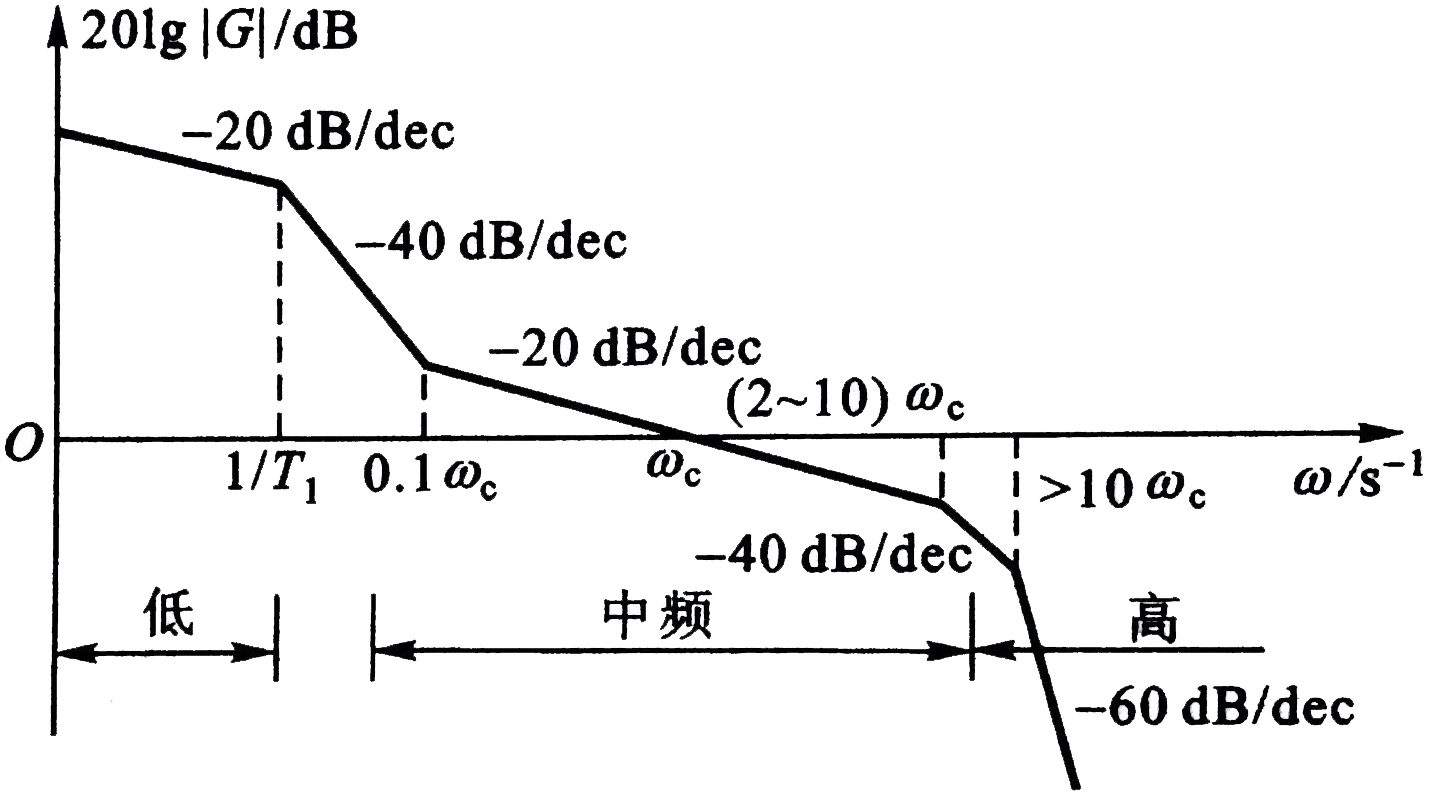
\includegraphics[width=0.53\linewidth]{pic/三频段.jpeg}
	\vspace*{-1em}
	\caption{系统开环Bode图}
	\label{开环Bode图}
\end{figure}
\begin{enumerate}[1. ]
	\item \dy[低频段]{DPD}
	\begin{itemize}
		\item 定义 \quad 通常是指$20\lg |G(\j\omega)|$的渐近曲线在第一个转折频率以前的区段。
		\item 特点 \quad 这一段的特性完全由积分环节和开环增益决定。
	\end{itemize}
	
	\item \dy[中频段]{ZPD}
	\begin{itemize}
		\item 定义 \quad 指$20\lg G(\j\omega)|$曲线在截止频率$\omega_{\text{c}}$附近的区段。
		\item 特点 \quad 这一段的特性集中反映了系统的平稳性和快速性。
	\end{itemize}
	
	\item \dy[高频段]{GPD}
	\begin{itemize}
		\item 定义 \quad 指$20\lg |G(\j\omega)|$曲线在中频段以后的区段$(\omega > 10\omega_{\text{c}})$。
		\item 特点 \quad 直接反映了系统对输入高频干扰信号的抑制能力。高频特性的分贝值越低,系统抗干扰能力越强。
	\end{itemize}
\end{enumerate}

\warn[
{
\begin{enumerate}
	\item 三频段的适用前提:\textcolor{red}{系统闭环稳定且具有最小相位性质的单位负反馈系统}。\vspace*{-0.5em}
	\item 三个频段的划分并无严格的确定准则,但是三频段的概念,为直接运用开环特性判别稳定的闭环系统的动态性能指出了原则和方向。\vspace*{0.5em}
\end{enumerate}
}
]






















 